
\section{Introduction}
%for reference to this section
\label{section:Introduction}
The purpose of this bachelor thesis research project is to provide information about the structure of modules over the locally finite Lie algebra $\mathfrak{sp}_{\infty}$.
Any finite-length module $M$ over a Lie algebra $\mathfrak{g}$ has well-defined socle and radical filtrations.
If these two filtrations coincide we say that the module $M$ is \textit{rigid}. 
The following questions about an arbitrary module are interesting: What are the socle and radical filtrations of $M$? What are the lengths of these filtrations? Is $M$ rigid? The answers to these questions help to estabilish links between these filtrations and other filtrations of $M$, and therefore can provide essential information on the structure of $M$.
\\We are interested in filtrations of the tensor modules of $\mathfrak{sp}_{\infty}$.
The results obtained in \cite{styrk}, \cite{weiss} and \cite{cohen} are going to be particularly influential in proving our main result. \cite{styrk} extends some results of Weyl to the classical locally finite Lie algebras $\mathfrak{gl}_{\infty}$, $\mathfrak{sl}_{\infty}$, $\mathfrak{sp}_{\infty}$ and $\mathfrak{so}_{\infty}$ and presents beautiful descriptions of the structure of their tensor representations. One of the most interesting results in \cite{styrk} is the decomposition of tensor representations of the classical locally finite Lie algebras $\mathfrak{gl}_{\infty}$, $\mathfrak{sp}_{\infty}$ and $\mathfrak{so}_{\infty}$ into indecomposable direct summands. Based on V.Serganova's observations, \cite{weiss} proves that some indecomposable direct summands of $\mathfrak{gl}_{\infty}$-tensor modules are non-rigid. In the paper \cite{styrk}, it is proven that the tensor modules of the classical locally finite Lie algebras $\mathfrak{gl}_{\infty}$ and $\mathfrak{sp}_{\infty}$ are injective. This beautiful argument is going to help us to show that some indecomposable direct summands of tensor representations of $\mathfrak{sp}_{\infty}$ are not rigid.
\\We started this project by studying the theory we need to understand the classical Lie algebra $\mathfrak{sp}_{\infty}$ and its tensor modules. Later we performed computations of their socle filtrations using the results from \cite{styrk}. The main results along with the computed diagrams are presented at the end of this paper.
\\Throughout this paper we are going to work over the field of complex numbers $\mathbb{C}$.
\section{Preliminaries}
We start our work by recalling the notions we will need about semisimple modules. Let $M$ be a module over a ring or a Lie algebra $R$.
\begin{defn}
$M$ is called \textbf{simple} if it has no proper submodules, and $M$ is called \textbf{semisimple} if it is a direct sum of simple submodules.
\end{defn}
\begin{defn}
Let $M$ be a nonzero module. $M$ is said to be \textbf{indecomposable} if
it cannot be expressed as a direct sum of two nonzero submodules. Otherwise it is called \textbf{decomposable}.
\end{defn}

\begin{thm}For any module $M$ the following statements are equivalent:
\begin{enumerate}[label=(\arabic*),ref=(\arabic*)]
\item $M$ is a direct sum of simple submodules.\label{statement1}
\item{ $M$ is the sum of all its simple submodules.}\label{statement2}
\item {Any submodule $N\subset M$ admits a direct complement in $M$ i.e  a submodule $K\subset M$} such that 
\\$M=N \oplus K.$\label{statement3}
\end{enumerate}
\end{thm}
\emph{Proof:} \Implies{statement1}{statement2} is obvious.
\\
\Implies{statement2}{statement3} Consider the set  $A$ of all submodules  of $M$ which intersect $N$ trivially

\begin{center}$A:=\{L\subset M $ | $ L\cap N=\{0\}\}.$
\end{center}
$A$ is non-empty since $\{0\}\in A$, $A$ is partially ordered by inclusion, and every chain of submodules in $A$ has an upper bound (the union of all submodules in the chain is an element of $A$). By Zorn's lemma, $A$ contains a maximal element $K$. By assumption, $M=\Sigma S_i$ for all simple submodules $S_i\subset M$. We claim that $N\oplus K=M$. Indeed, if there is a simple submodule $S\subset M$ such that $S\not\subset N\oplus K$, then $(N\oplus K) \cap S=\{0\}$ by the simplicity of $S$. Hence, $(S+K)\cap N=\{0\}$, therefore $S+ K$ is contained in $A$. On the other hand, $S+K$ properly contains $K$, which contradicts the maximality of $K$.
\\
\Implies{statement3}{statement1} First we show that a stronger version of (3) applies: if $N\subset M$ is a submodule, then for every submodule $L\subset N$ there exists a submodule $L'\subset N$ such that $L\oplus L'=N$. Indeed, as $L\subset M$, $L$ has a complement $L''$ in $M$, i.e, $L\oplus L''=M$. Consider $L'=L''\cap N \subset L''$. Then $L'\cap L=\{0\}$ and $L'+L=N$. 
Therefore, $N=L'\oplus L$.
\\
Now consider 
\begin{center}
$B:=\{L\subset M$ | $ L=\oplus S_i$ where $S_i\subset L$ are simple$\}$.\end{center}
The set $B$ is non-empty and is partially ordered: $L=\oplus S_i <L'=\oplus S'_i$ if for any $i$, there exists $i'$ such that $S_i=S'_i$. Moreover, Zorn's condition is clearly satisfied. Applying Zorn's lemma to $B$ yields a maximal element $K$ of $B$. We claim that $K=M$. Indeed, if $K\subsetneq M$, by (3) there is $N\subset M$ such that $K\oplus N=M$. If $N$ contains a simple submodule $N'\subset N$, then $K\oplus N' \in B$, contradicting the maximality of $K$.
\\Therefore, in order to finish the proof we need to show that $N$ contains a simple submodule. If $N$ is simple there is nothing to prove. If $N$ is not simple, fix a nonzero $x\in N$ such that $$C:=\{P\subset N| P \textnormal{ is nonzero and } P\not\ni x\}$$ is non-empty. Then $C$ is ordered by inclusion and satisfies Zorn's condition. Let $Y$ be a maximal element of $C$. Then $N=X\oplus Y$ for some submodule $X\subset N$. Clearly, $X$ is generated by $x$. But then $X$ is simple as otherwise $Y\oplus X'\in C$ for any submodule $X'\subset X$,  $x\not \in X'$. This shows that $N$ contains a simple submodule, and the proof is complete. $\blacksquare$

\subsection{Loewy filtrations}
Let $M$ be an $R-$module.
\begin{defn}
A \textbf{filtration} of $M$ is a chain of nested submodules of $M$
\begin{equation}
\dots \subset M_i\subset M_{i+1} \subset \dots
\end{equation}
A filtration is called \textbf{finite} if there are only finitely many distinct modules in the set $\{M_i\}$. The number of distinct non-zero proper submodules of $M$ in the chain (1) is called the \textbf{length} of the filtration.
\end{defn}
\begin{defn}
A filtration is \textbf{semisimple} if the quotients $M_{i+1}/M_{i}$ are semisimple whenever nonzero.
\end{defn}
In this research we are interested only in semisimple filtrations.\\ 
\begin{defn}
We call a finite filtration of $M$ a \textbf{Loewy filtration} if there is no semisimple finite filtration of $M$ with smaller length.
\end{defn}
Below we are going to give important examples of Loewy filtrations.
\\ \\Let $R$ be a $\mathbb{C}$-algebra and $M$ be an $R$-module. 
\begin{defn}
The \textbf{socle} of $M$ is defined to be the largest semisimple submodule of $M$, in other words, $soc M$ is the sum of all simple submodules of $M$. If there are no simple submodules of $M$, we set $socM=0$.
\end{defn}
We define $soc^0 M:=0$, $soc^1 M:=socM$, and $soc^iM:= \pi_{i}^{-1}(soc(M/soc^{i-1}M))$, where $\pi_{i}:M \rightarrow M/soc^{i}M$, for $i\in\mathbb{Z}_{>0}$. One can see that the following holds $$soc^{i}M/soc^{i-1}M=soc(M/soc^{i-1}M),$$ and it implies that the quotients $soc^{i}M/soc^{i-1}M$ are semisimple. Then the following semisimple filtration of $M$ is called the \textbf{socle filtration} of $M$
$$0=soc^0M\subset soc^1M\subset \dots .$$
The quotients are called the\textbf{ socle layers} and are denoted as
$$\overline{soc^i M}=soc^{i}M/soc^{i-1}M.$$
\begin{defn}
The \textbf{radical} of $M$ is the smallest submodule $N$ of $M$ such that the quotient $M/N$ is semisimple.
\end{defn}
 One could also verify that the following is true for the radical of a module $M:$ $$rad M=\bigcap_{\Phi:M\rightarrow W}ker\Phi,$$
where $\Phi$ denotes a homomorphism from $M$ to an arbitrary semisimple $R$-module $W$. We define $rad^0M:=M$, $rad^{i+1}M:=rad(rad^iM)$,  for $i\in\mathbb{Z}_{>0}$. It follows that the quotients $rad^iM/rad^{i+1}M$ are semisimple and we obtain the following filtration of $M$:
$$\dots \subset rad^2M \subset rad^1M\subset rad^0M=M.$$
This filtration is called the \textbf{radical filtration} of $M$, if for some $n\in\mathbb{Z}_{>0}$, $rad^nM=0$.
The quotients of consecutive submodules are called the \textbf{radical layers} and are denoted as $$\overline{rad^{i+1}M}:=rad^iM/rad^{i+1}M.$$
The following theorem explains the relation between the socle and radical filtrations of a given module:

\begin{thm}
Let $M$ be a module over a ring or a Lie algebra $R$ and suppose that one of the following holds for some $n\in \mathbb{Z}^{+}$
 \begin{itemize}
 \item{$soc^n M=M,$}
 \item{$\textnormal{rad}^n M=0$}
 \end{itemize}
 but neither holds for any smaller n. Then the other equation is also true and the filtrations satisfy
 $$\textnormal{rad}^{n-i} M \subseteq soc^i M$$
 for all  \hspace{1mm}$0\leq i \leq n$.
 In other words, if one of the filtrations exhausts $M$ after a finite number of steps, then both filtrations are finite and have the same length. This length is called the \textbf{Loewy length} of $M$.
\end{thm}
\emph{Proof:} Assume $soc^nM=M$. We apply induction on the length of socle filtration of $M$. For $i=0$, $ rad^{0}M=M=soc^nM$. Suppose that for some $0<k<n $, $ rad^kM\subseteq soc^{n-k}M$. Then,

$$rad^{k+1}M=\bigcap_{\Phi:rad^kM\rightarrow W}ker\Phi\subseteq \bigcap_{\Phi:soc^{n-k}M\rightarrow W}ker\Phi$$

The map $\pi:soc^{n-k}M\rightarrow (soc^{n-k}M)/(soc^{n-k-1}M)$ is a homomorphism with a semisimple module as its codomain (the socle layers are semisimple). Therefore,
$$rad^{k+1}M\subseteq ker\pi=soc^{n-k-1}M.$$Hence, we have proven that $rad^{n-i}M\subseteq soc^i M$ for all positive integers $0\le i\le n$. In particular, $rad^nM\subseteq soc^{0}M=0$. 
\vspace{2mm}
\\Now assume $rad^nM=0$. We apply induction on the length of the radical filtration of $M$. It is obvious that $rad^nM=0=soc^0M$. Suppose that $rad^kM\subseteq soc^{n-k}M$ for some positive integer $0<k<n$. Consider the homomorphisms
$\pi_1:M/rad^kM\rightarrow M/soc^{n-k}M$, $\pi_2:M\rightarrow M/rad^{k}M$ and $\pi:M\rightarrow M/soc^{n-k}M$. Clearly, $\pi=\pi_1 \circ\pi_2$.
By definition, $$soc^{n-k+1}M=\pi^{-1}(soc(M/soc^{n-k}M)).$$
On the other hand, $$rad^{k-1}M\subseteq \pi_{2}^{-1}(rad^{k-1}M)/(rad^kM)=\pi_{2}^{-1}(\pi_{1}^{-1}(soc(M/soc^{n-k}M)))=\pi^{-1}(soc(M/soc^{n-k}M)).$$
It follows that $rad^{k-1}M\subseteq soc^{n-k+1}M,$ which implies that
$$rad^{i}M\subseteq soc^{n-i}M$$ for all positive integers $0\leq i\leq n$. Moreover, $M=rad^0M\subseteq soc^{n}M$, therefore $ M=soc^nM$. $\blacksquare$
\\Under the assumption of Theorem 2.2 both the radical and socle filtrations of a module $M$ are Loewy filtrations. Their length coincide and is called the \textit{Loewy length} of $M$. If the radical and socle filtrations of $M$ coincide, we say that $M$ is a \textbf{rigid} module.

\subsection{Tensor representations of  $\mathfrak{gl}_{\infty}$ and $\mathfrak{sp}_{\infty}$ }
In this section we define the infinite dimensional locally finite Lie algebras $\mathfrak{gl}_{\infty}$ and $\mathfrak{sp}_{\infty},$ and introduce their tensor representations. 


\normalsize In order to describe the tensor representations of $\mathfrak{sp}_{\infty}$ first we need to understand  the tensor representations of $\mathfrak{gl}_{\infty}$. For this reason I am going to review some results from \cite{styrk}.\\ \\Let $V$ and $V_*$ be countable dimensional vector spaces and $\langle \cdot,\cdot \rangle : V \otimes V_{*} \rightarrow \mathbb{C}$ be a non-degenerate pairing. The Lie algebra $\mathfrak{gl}_\infty$ is defined as the vector space $V\otimes V_{*}$ endowed with the Lie bracket satisfying
\begin{equation}
[u\otimes u^{*},v\otimes v^{*}]=\langle v, u^*\rangle u\otimes v^*-\langle u,v^*\rangle v \otimes u^*
\end{equation}
for $u,v\in V \textnormal{ and } u^*,v^* \in V^*$.
G. Mackey \cite{mackey} has proven that one can find dual bases $ \{\xi_i\}_{i \in J}$ of $V$ and $\{\xi^{*}_i\}_{i \in J}$ of $V_*$, where $J=\mathbb{Z}/\{0\}$, such that we have  $\langle \xi_i , \xi_{j}^{*} \rangle=\delta_{i,j}$. Given such a basis of $V$ we can think of $\mathfrak{gl}_{\infty}$ as the Lie algebra with linear basis $\{E_{i,j}=\xi_i \otimes \xi_{j}^{*}| $ $i,j\in J \}$. Then $(2)$ becomes $$[E_{i,j},E_{k,l}]=\delta_{k,j}E_{i,l}-\delta_{i,l}E_{k,j}.$$
We call $V$ the \emph{natural representation} of $\mathfrak{gl}_{\infty}$, and $V_*$ the conatural representation of $V$.\\ \\For integers $p,q>0$ the tensor representation $V^{\otimes(p,q)}$ is defined as $V^{ \otimes p} \otimes(V _{*})^{\otimes q}$ and is equipped with a $\mathfrak{gl}_{\infty}$-module structure satisfying
$$(u\otimes u^*)(v_1 \otimes \dots \otimes v_p \otimes v_1^{*}\otimes\dots \otimes v_q^{*})=
\Sigma_{i=1}^{p}\langle v_i,u^*\rangle v_1 \otimes \dots  \otimes v_{i-1}\otimes u \otimes v_{i+1} \otimes \dots \otimes v_p\otimes v_1^*\otimes \cdots \otimes v_q^* -$$
$$\Sigma_{j=1}^{q}\langle u, v_j^*\rangle v_1\otimes\dots \otimes v_p\otimes v_1^*\otimes v_{j-1}^*\otimes u^* \otimes v_{j+1}^* \otimes \dots \otimes v_q^*$$ for $u,v_1, \dots, v_p \in V$ and $u^*,v_1^*,\dots, v_q^*\in V_*.$\\ \\The product of symmetric groups $\mathfrak{S}_p \times \mathfrak{S}_q$ acts on $V^{\otimes(p,q)}$ by permuting the factors, and this action commutes with the action of $\mathfrak{gl}_{\infty}$ on $V^{\otimes (p,q)}$. For this reason we say that $V^{\otimes (p,q)}$ is a $(\mathfrak{gl}_{\infty},\mathfrak{S}_p\times \mathfrak{S}_q)$-module.
\\For any pair of indices $I=(i,j)$ such that $i\in\{1, \dots ,p\}$ and $j\in \{1,\dots,q\}$ we consider a tensor contraction
$$\Phi_{I}:V^{\otimes (p,q)}\rightarrow V^{\otimes(p-1,q-1)}$$ such that $v_1\otimes\dots \otimes v_p\otimes v_1^*\dots\otimes v_q^*\mapsto \langle v_i,v_j^*\rangle v_1 \otimes \dots \otimes \hat{v_i}\otimes \dots \otimes \hat{v_j}^* \otimes \dots \otimes v_q^* $, where $\hat{v_i}$ and $\hat{v_j^{*}}$ means that these terms are left out.\\ 
\\We define the $(\mathfrak{gl}_{\infty},\mathfrak{S}_p\times \mathfrak{S}_q)$ submodule $V^{\{p,q\}}$ of $V^{\otimes(p,q)}$ as
$$V^{\{p,q\}}:= \bigcap_{I}  ker(\Phi_I : V^{\otimes (p,q)} \rightarrow V^{\otimes(p-1,q-1)} ),$$ and we set $V^{\{p,0\}}:=V^{\otimes p}$ and 
$V^{\{0,q\}}:=V^{\otimes q}$ whenever $p=0$ or $q=0$.
\\Now we are ready to define the simple finitary Lie algebra $\mathfrak{sp}_{\infty}$.
\\Let $V$ be a countable dimensional vector space and $\Omega : V\otimes V\rightarrow \mathbb{C}$ be a non-degenerate anti-symmetric bilinear form on $V$. Then the Lie algebra $\mathfrak{sp}_{\infty }$ is defined as the Lie subalgebra of $\mathfrak{gl}_{\infty}$ under which the bilinear form $\Omega$ is invariant. In other words,
$$\mathfrak{sp}_{\infty}=\{g\in \mathfrak{gl}_{\infty} |\hspace{1mm}\Omega(gu,v)+\Omega(u,gv)=0\}$$ for all $u,v \in V$.
Similarly to the case $\mathfrak{gl}_{\infty},$ based on an observation of Mackey we can pick a basis $\{\xi_i\}_{i \in \mathbb{Z}/\{ 0 \}}$ of $V$, such that, $\Omega(\xi_i,\xi_j)=sgn(i)\delta_{i+j,0}$.\\ \\ We can also view $\mathfrak{sp}_{\infty }$ as the Lie algebra with linear basis 
$\{sgn(j) E_{i,j}-sgn(i)E_{-j,-i}\}$, where $E_{i,j}=\{\xi_i\otimes \xi_j| i,j \in J\}$. In this case the dual basis is $\xi_i^*=sgn(i)\xi_i$, therefore $\mathfrak{sp}_{\infty}=Sym^2V$.
\\ \\We call $V$, considered as an $\mathfrak{sp}_{\infty}$-module by restriction, the \emph{natural representation} of $\mathfrak{sp}_{\infty}$. Since $V\cong V_{*}$ as $\mathfrak{sp}_{\infty}$-modules, the $\mathfrak{sp}_{\infty}$- action on the $\mathfrak{gl}_{\infty}$-module $V^{\otimes(p,q)}$ coincides with the $\mathfrak{sp}_{\infty}$-action on the $\mathfrak{gl}_{\infty}$-module $V^{\otimes(p+q)}$. For this reason it suffices to study the  tensor representations $V^{\otimes d}$. In other words, we are going to study the decomposition of $V^{\otimes d}$ into a direct sum of indecomposable submodules. As we will see later, the irreducible subquotients of these indecomposable $\mathfrak{sp}_{\infty}$-modules are highest weight modules.\\
\\Now we consider a tensor contraction for any pair of indices $I=(i,j)$ such that $i,j\in\{1,\dots,d\}$
 $$\Phi_{\langle I\rangle}:V^{\otimes d}\rightarrow V^{\otimes(d-2)},$$
$$v_1\otimes\dots \otimes v_d \mapsto \Omega(v_i,v_j)v_1 \otimes\dots \otimes \hat{v_i}\otimes \dots \otimes \hat{v_j} \otimes \dots \otimes v_d. $$
\\Furthermore, we define $V^{\langle 0 \rangle}:=\mathbb{C}$ and $V^{\langle 1 \rangle}:=V$ and $$V^{\langle d \rangle}:= \bigcap_{I} ker(\Phi_{\langle I\rangle} : V^{\otimes d} \rightarrow V^{\otimes(d-2)} )$$
for all positive integers $d\geq 2 $.

\subsection{Young tableaux and Schur functors}
\begin{defn}
Given a positive integer $d$, we define a \textbf{partition} $\lambda$ of $d$ to be a sequence of positive integers
$$\lambda=(\lambda_1,\lambda_2,\dots,\lambda_k)  \textnormal{  such that   } \lambda_1\geq \lambda_2\geq\dots\geq\lambda_k  >0\textnormal{  and  }d=|\lambda|:=\Sigma_{1}^{k}\lambda_i.$$   We call $k$ the \textbf{length} of the partition $\lambda$.
\end{defn}
To each partition $\lambda=(\lambda_1,\lambda_2,\dots,\lambda_k)$ of a positive integer $d$, one associates a \textbf{Young diagram} which has $k$ rows and $\lambda_i$ boxes in the $i$ th row, the rows being lined up on the left.
\\
\begin{center}
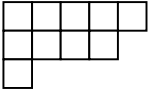
\includegraphics[width=4cm]{Young.png}
\\
\vspace{2 mm}
\textbf{Figure 1} Young diagram of the partition $(5,4,1)$
\end{center}
The \emph{conjugate} of a partition $\lambda$ is the partition $\lambda^{T}$ associated to the Young diagram obtained by transposition of the Young diagram of $\lambda$. The importance of partitions in representation theory is that they parametrize the irreducible representations of $\mathfrak{S}_d$.
\\A\textbf{ Young tableau} is a Young diagram in which boxes are filled with the numbers from $1$ to $|\lambda|$.
\\Given a Young tableau of $\lambda$, where $|\lambda|=d$, we can define two subgroups of the symmetric group
$$P=P_\lambda:=\{g\in \mathfrak{S}_d | \textnormal{ g preserves each row}\},$$
$$Q=Q_\lambda:=\{h\in \mathfrak{S}_d |  \textnormal{ $h$ preserves each column}\}.$$ Consider two elements in the group algebra $\mathbb{C}\mathfrak{S}_d$:
$$a_{\lambda}=\Sigma_{g \in P} e_g \textnormal{, } b_{\lambda}=\Sigma_{h\in Q}sgn(h) \cdot e_h.$$
If $V$ is a vector space over $\mathbb{C}$, and $\mathfrak{S}_d$ acts on $V^{\otimes d}$ by permuting the factors, the image of 
\\$a_\lambda : V^{\otimes d} \rightarrow V^{\otimes d}$ is the following subspace of $V^{\otimes d}$: $$Im(a_\lambda)=Sym^{\lambda_1}V\otimes Sym^{\lambda_2}V\otimes \dots \otimes Sym^{\lambda_k}V$$Similarly, the image of $b_\lambda$ is the following subspace of $V^{\otimes d}$: $$Im(b_\lambda)={\bigwedge}^{\mu_1}V\otimes {\bigwedge}^{\mu_2}V\otimes\dots \otimes  {\bigwedge}^{\mu_n}V$$where $\mu$ is the partition conjugate to $\lambda$. We define the Young symmetrizer $c_{\lambda}$ by setting: $$c_\lambda=a_\lambda \cdot b_\lambda \in \mathbb{C}\mathfrak{S}_d.$$
If we define $$H_{\lambda}:=\mathbb{C}[\mathfrak{S}_{d}]c_{\lambda},$$then $H_{\lambda}$ is an irreducible representation of $\mathfrak{S}_{d}.$ It can be shown that every irreducible representation of $\mathfrak{S}_{d}$ is isomorphic to $H_{\lambda}$ for some $\lambda$ with $|\lambda|=d.$
\\We can also see that $c_\lambda$ projects $V^{\otimes d}$ onto $$\mathbb{S}_\lambda V:=im(c_\lambda:V^{\otimes d} \rightarrow V^{\otimes d})$$ which is  an irreducible representation of $\mathfrak{gl}_{n}$. Here $\mathbb{S}_\lambda$ is called the Schur functor corresponding to a partition $\lambda$. More on this can be found in \cite{fulton}. 


\subsection{Highest weight modules }
In order to give a concrete construction of tensor representations of $\mathfrak{sp}_{\infty}$, we need to review some background material. 
\begin{defn}
Let $\mathfrak{g}$ be a Lie algebra. Then $x\in\mathfrak{g}$ is said to be semisimple if $ad x$ is semisimple (i.e the adjoint map of x is diagonalizable).
\end{defn}
\begin{defn}
A Lie subalgebra of $\mathfrak{g}$ is said to be \textbf{toral} if it entirely consists of semisimple elements. 
\end{defn}
Let $M$ be a $\mathfrak{g}$-module, $\mathfrak{t}$ be a toral subalgebra of $\mathfrak{g}$, and $\mathfrak{t}^{*}$ be its dual.
For each $\alpha\in \mathfrak{t}^{*}$ let:
$$M^{\alpha}:=\{v\in M|tv=\alpha(t)v \hspace{2mm} \forall t\in \mathfrak{t}\}.$$
The space $M^{\alpha}$ is the space of \textit{weight vectors of weight} $\alpha.$
If $M^{\alpha}\neq 0$, we say that $\alpha$ is a \textit{weight} of $M$. It can be verified that weight vectors for distinct weights in $M$ are linearly independent, therefore $\Sigma_{\alpha\in \mathfrak{t}^{*}} M^{\alpha}$ is a direct sum and $\Sigma_{\alpha\in \mathfrak{t}^{*}} M^{\alpha}\subseteq M$. We call $M$ a $\mathfrak{t}$-\textit{weight $\mathfrak{g}$-module}  if $\Sigma_{\alpha\in \mathfrak{t}^{*}} M^{\alpha}=M$. 
\\In what follows $\mathfrak{g}=\mathfrak{gl}_{\infty}, \mathfrak{sp}_{\infty}.$
\begin{defn}
A \textbf{splitting Cartan subalgebra} $\mathfrak{h}$ of $\mathfrak{g}$ is a maximal toral subalgebra such that $\mathfrak{g}$ is an  $\mathfrak{h}$-weight module.
\end{defn}
If $\mathfrak{h}$ is a splitting Cartan algebra, then $\mathfrak{g}$ is an $\mathfrak{h}$-weight module:
$$\mathfrak{g}=\mathfrak{h}\oplus\bigoplus_{\alpha\in{\mathfrak{h}}^{*}/\{0\}}\mathfrak{g}^{\alpha}.$$
This decomposition of $\mathfrak{g}$ is called the \textbf{root decomposition} of $\mathfrak{g}$ with respect to the Cartan subalgebra $\mathfrak{h}$. The nonzero spaces $\mathfrak{g}^{\alpha}$ for $\alpha\ne 0$ are called the \textbf{root spaces} of $\mathfrak{g}$ and $\Delta:=\{\alpha \in \mathfrak{h}^{*}/\{0\}$ | $\mathfrak{g}^{\alpha}\ne 0\}$ is called the \textbf{set of roots} of $\mathfrak{g}^{\alpha}$.
The decomposition of the set $\Delta$ into two disjoint sets $\Delta^{+}$ and $\Delta^{-}$ is called a \textbf{triangular decomposition} of $\Delta$ if and only if $\alpha,\beta \in \Delta^{+}$, $\alpha+\beta\in \Delta$ implies $\alpha+\beta \in{\Delta^{+}}$, and $\alpha\in\Delta^{\pm}$ implies $-\alpha\in\Delta^{\mp}$.
\\
\begin{defn}
A Lie subalgebra $\mathfrak{b}$ of $\mathfrak{g}$ is called a \textbf{Borel subalgebra} if there is a triangular decomposition such that $\mathfrak{b}=(\bigoplus_{\alpha\in\Delta^{+}}\mathfrak{g}^{\alpha})\rtimes\mathfrak{h}.$ 
\end{defn} 

\begin{defn}
Let $M$ be a $\mathfrak{g}$-module and $\mathfrak{b}\subset\mathfrak{g}$ be a Borel subalgebra.
If $v\in M$ and $v$ generates a one-dimensional $\mathfrak{b}$-submodule, then we call $v$ a  \textbf{$\mathfrak{b}$-singular vector}.
\end{defn}
It follows that any such vector satisfies $(\bigoplus_{\alpha\in\Delta^{+}}\mathfrak{g}^{\alpha})v=0$ and for all, $ x\in\mathfrak{h}$,  $x v=\chi(x)v$ for some fixed \textit{weight} $\chi \in \mathfrak {h}^{*}$.
\begin{defn}
A module $M$ is called a \textbf{highest weight module} if it is generated by some $\mathfrak{b}$-singular vector $v$ of weight $\chi\in \mathfrak{h}^{*}.$ The weight $\chi$ is called the \textbf{highest weight} of $M$.
\end{defn}
It is a straightforward fact that the highest weight vector $v$ of $M$ is determined uniquely up to scalar multiplication. Moreover, a highest weight module is always a weight module.
\\When $\mathfrak{g}=\mathfrak{gl}_{\infty}$, we have the following root decomposition:
$\mathfrak{gl}_{\infty}=\mathfrak{h}\oplus(\bigoplus_{\alpha\in\Delta}\mathbb{C}X_{\alpha})$, where 
$$\mathfrak{h}_{\mathfrak{gl}}=\bigoplus_{i\in J}\mathbb{C}E_{i,i},\hspace{5mm} \Delta_{\mathfrak{gl}}=\{\epsilon_i-\epsilon_j|i,j\in J, i\ne j\},\hspace{5mm} X^{\mathfrak{gl}}_{\epsilon_i-\epsilon_j}=E_{i,j}$$ 
and $\epsilon_{i}\in \mathfrak{h}^{*}$ is determined by $\epsilon_{i}(E_{j,j})=\delta_{i,j}$. Here $J$ is a countable set. If we put $J=\mathbb{Z}/\{0\}$, we can define the following triangular decomposition
\begin{equation}
\Delta^{+}=\{\epsilon_i-\epsilon_j|0<i<j\}\cup\{\epsilon_i-\epsilon_j|i<j<0\}\cup\{\epsilon_i-\epsilon_j|j<i<0\}, \textnormal{ } \Delta^{-}=-\Delta^{+}.
\end{equation}
\begin{defn}
For any partitions $\lambda$ and $\mu$ such that $|\lambda|=p$ and $|\mu|=q$, we define the $\mathfrak{gl}_{\infty}$-submodule  $\Gamma_{\lambda,\mu}$ of $V^{\{p,q\}}$ by setting
$$\Gamma_{\lambda,\mu}:=V^{\{p.q\}}\cap (\mathbb{S}_{\lambda}V\otimes \mathbb{S}_{\mu}V_{*}).$$
\end{defn} 
With respect to the Borel subalgebra $\mathfrak{b}$ determined by (3), $\Gamma_{\lambda,\mu}$ is an irreducible highest weight $\mathfrak{gl}_{\infty}$-module. It was shown in \cite{styrk} that as an $\mathfrak{sp}_{\infty}$-module, $\Gamma_{\lambda,0}$ is not a highest weight module, but only an indecomposable module.
\\Now let us explore $\mathfrak{sp}_{\infty}$, the simple locally finite Lie algebra we are interested in. It has the following root decomposition:
$$\mathfrak{sp}_{\infty}=\mathfrak{h}_{\mathfrak{sp}}\oplus(\bigoplus_{\lambda \in \Delta_{\mathfrak{sp}}}\mathbb{C} X_{\lambda}^{\mathfrak{sp}}),$$
where
$$\mathfrak{h}_{\mathfrak{sp}}=\bigoplus_{i\in \mathbb{Z}_{>0}}(E_{i,i}-E_{-i,-i}),\hspace{5mm} \Delta_{\mathfrak{sp}}=\{\pm(\epsilon_i+\epsilon_j)|i,j\in\mathbb{Z}_{>0}\}\cup\{(\epsilon_{i}-\epsilon_{j})|i,j\in\mathbb{Z}_{>0} \textnormal{ and } i\ne j\}$$ 
$$X^{\mathfrak{sp}}_{\epsilon_i+\epsilon_j}=E_{i,-j}+E_{j,-i},\hspace{5mm}X^{\mathfrak{sp}}_{-\epsilon_i-\epsilon_j}=E_{i,j}+E_{-j,i},\hspace{5mm}X^{\mathfrak{sp}}_{\epsilon_i-\epsilon_j}=E_{i,j}+E_{-j,-i}.$$
Here $\{E_{i,j}\}$ is the basis of $\mathfrak{gl}_{\infty}$, and  $\epsilon_{i}\in \mathfrak{h}_{\mathfrak{sp}}^{*}$ is defined by the equality  $\epsilon_{i}(E_{j,j}-E_{-j,-j})=\delta_{i,j}$ for $i,j\in \mathbb{Z}_{>0}$.
\vspace{2mm}
\\In this case we fix the following Borel subalgebra of $\mathfrak{sp}_{\infty}$: $$\mathfrak{b}=(\bigoplus_{\lambda\in\Delta^{+}_{\mathfrak{sp}}}\mathfrak{sp}_{\infty}^{\lambda})\oplus\mathfrak{h}_{\mathfrak{sp}} \textnormal{  where  } \Delta_{\mathfrak{sp}}^{+}=\{ (\varepsilon_j+\varepsilon_i)|i,j\in\mathbb{Z}_{>0} \textnormal{ and }i \geq j \}\cup \{(\varepsilon_i-\varepsilon_j)|i,j\in\mathbb{Z}_{>0} \textnormal{ and } i< j\}. $$
\\For any partition $\lambda$ such that $|\lambda|=d$, we define the $\mathfrak{sp}_{\infty}$-submodule $\Gamma_{\langle \lambda \rangle}$ of $V^{\otimes d}$ as
$$\Gamma_{\langle \lambda \rangle}:=V^{\langle d \rangle} \cap \mathbb{S}_{\lambda}V.$$
\\It turns out that $\Gamma_{\langle\lambda\rangle}$ is an irreducible highest weight $\mathfrak{sp}_{\infty}$-module.
We proceed to find out more about this and some other known results from \cite{styrk} about the structure of $\mathfrak{sp}_{\infty}$.

\section{Results about tensor representations of $\mathfrak{sp}_{\infty}$}
The following theorem from \cite{styrk} states in particular that $\Gamma_{\langle\lambda\rangle}$ is an irreducible highest weight $\mathfrak{sp}_{\infty}$-module.
\begin{thm}

For any non-negative integer $d$ there is an isomorphism of $(\mathfrak{sp}_{\infty},\mathfrak{S}_p)$-modules
$$V^{\langle d\rangle}\cong \bigoplus_{|\lambda|=p}\Gamma_{\langle \lambda\rangle} \otimes H_{\lambda}$$For every partition $\lambda$, the $\mathfrak{sp}_{\infty}$-module  $\Gamma_{\langle \lambda \rangle}$ is an irreducible highest weight module with highest weight $\omega=\Sigma_{i\in\mathbb{N}}\lambda_{i}\epsilon_{i}.$
\end{thm}
The following fact will be very important for the main result of this project:
\begin{lem}
Any automophism $\phi$ of the $\mathfrak{sp}_{\infty}$-module \textit{ $\Gamma_{\langle\lambda\rangle}$} is of the form $\phi(v)=cv$, where $c\in \mathbb{C}\setminus\{0\}.$
\end{lem}
\emph{Proof: } Since $\Gamma_{\langle\lambda\rangle}$ is a highest weight module, it is generated by some $\mathfrak{b}$-singular vector $v\in \Gamma_{\lambda}$ which is unique up to a scalar multiplication. Therefore any automorphism $\phi$ sends $v$ to $cv$ where $c$ is a nonzero complex number. Since $v$ generates $\Gamma_{\langle\lambda\rangle}$, $\phi$ is already determined uniquely by $c$. Hence, $\phi(v)=cv$ for every $v\in\Gamma_{\langle\lambda\rangle} $.$\blacksquare$
\\Next we restate the theorem from \cite{styrk} that describes the socle filtrations of the tensor representations of $\mathfrak{sp}_{\infty}$.
\begin{thm}
For any non-negative integer $d$ the $\mathfrak{gl}_{\infty}$-module $V^{\otimes d} $, regarded as an $\mathfrak{sp}_{\infty}$-module, has Loewy length $[\frac{d}{2}]+1$, and
$$soc^{r}V^{\otimes d}=\bigcap_{I_1,I_2,\dots,I_r}ker(\Phi_{\langle I_1, I_2, \dots I_r\rangle}:V^{\otimes p}\rightarrow V^{\otimes(d-2r)}),\hspace{5mm} r=1,2,\dots [\frac{d}{2} ],$$ where $\Phi_{\langle I_1, I_2, \dots I_r\rangle}:= \Phi_{I_1} \circ \Phi_{I_2} \circ \dots \circ \Phi_{I_r}.$
\end{thm}
This result can be used to obtain the following theorem which describes the socle filtration of each indecomposable direct summand $\Gamma_{ \lambda}$.
\begin{thm}
For any partition $\lambda$, the $\mathfrak{sp}_{\infty}$-module $\Gamma_{\lambda}$ is indecomposable and
$$\overline{soc}^{r+1}\Gamma_{\lambda}\cong \bigoplus_{|\mu|=|\lambda|-|2\gamma|} (\Sigma_{|\gamma|=r}N^{\lambda}_{\mu,(2\gamma)^{T}})\Gamma_{\langle \mu \rangle}, \hspace{5mm} r=1,\dots,[ \frac{d}{2}].$$
\end{thm}
The coefficients $N^{\lambda}_{\mu,(2\gamma)^{T}}$ are called \textit{Littlewood-Richardson coefficients} and we are going to learn more about them in the next section.


\subsection{Littlewood-Richardson coefficients}
\normalsize 
The Littlewood-Richardson coefficients are very important when studying the socle filtrations of indecomposable direct summands of $V^{\otimes d}$.
\vspace{2mm}
\\ The \textbf{Littlewood-Richardson coefficients} $N^{\lambda}_{\mu,\gamma}$ are non-negative integers which depend on three partitions $\lambda, \mu, \gamma$ and are determined by relation
$$S_{\mu}S_{\gamma}=\Sigma_{\lambda}N^{\lambda}_{\mu,\gamma}S_{\lambda},$$
where $S_{\mu}$ is the Schur symmetric polynomial corresponding to the partition $\mu$. For more details on this relation see \cite{fulton} pages 455-456.\\ \\Let $\lambda \textnormal{ and }\mu$ be partitions such that $\lambda_i\ge\mu_i$ for each $i$. Consider a partition $\gamma$ such that $|\gamma|=|\lambda|-|\mu|$.\\ \\We call the set-theoretic difference of the Young diagrams of $\lambda$ and $\mu$   a \emph{skew diagram} of shape  $\lambda/\mu$. A \emph{semistandard skew} tableau of shape $\lambda/\mu$  and weight $\gamma$ is a skew diagram filled with numbers that satisfies the following conditions:
\begin{itemize}
\item{each positive integer $i$ less than or equal to $|\gamma|$ appears exactly $\gamma_{i}$ times,}
\item{the numbers along each column are strictly increasing,}
\item{the numbers along each row are weakly increasing.}
\end{itemize}
If in addition the following condition holds
\begin{itemize}
\item{after removal of 1 or more leftmost columns we again obtain a semistandard skew tableau,}
\end{itemize}
we call such a semistandard skew tableau a \textbf{Littlewood-Richardson tableau}.\\ 
\begin{thm}{(Littlewood-Richardson Rule)}
For partitions $\lambda,\mu,\gamma$, the Littlewood-Richardson coefficient $N^{\lambda}_{\mu,\gamma}$ is equal to the number of Littlewood-Richardson tableaux of shape $\lambda/\mu$ and of weight $\gamma$.
\end{thm}

\begin{center}
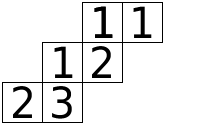
\includegraphics[width=3cm]{Download.png}
\hspace{3mm}
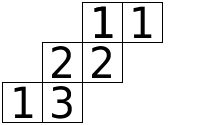
\includegraphics[width=3cm]{Download__1_.png}

\vspace{2 mm}

\textbf{Figure 2} There are only 2 Littlewood-Richardson tableaux of shape $(4,3,2)/(2,1)$ and of weight $(3,2,1)$ therefore $ N^{(4,3,2)}_{(2,1),(3,2,1)}=2$
\end{center}
More information on this theorem can be found in \cite{fulton}. The following observation is very easy to verify and is going to be very helpful later.
\\If $\lambda$ is a partition of length 1, i.e $\lambda=(d)$ where $d\in \mathbb{Z}^{+}$, then $N_{\mu,\gamma}^{\lambda}\neq 0$ if and only if $\gamma$ is of length 1 i.e $\gamma=(d')$ for some $d'\in \mathbb{Z}^{+}$ such that $d'<d$.
\


\section{Main results}
\subsection{Non-rigidity of the tensor representations of $\mathfrak{sp}_{\infty}$ and their indecomposable direct summands}
A first observation is that any tensor representation $V^{\otimes d}$ of $\mathfrak{sp}_{\infty}$ is non-rigid. Indeed, note that the Loewy length of the indecomposable direct summand of $V^{\otimes d}$ corresponding to the partition $(d)$ of $d$ is $1$. On the other hand, Theorem 3.4 implies that the remaining indecomposable direct summands are of Loewy length at least $2$. Hence, the socle filtration of an arbitrary tensor module $V^{\otimes d}$ does not coincide with its radical filtration. The following example illustrates this argument:

\begin{center}
$V^{\otimes 2} \sim    $ 
 \begin{tabular}{ |l| }
  \hline
   \\
  \hline
  $\Gamma_{\langle(2)\rangle}$
  \\ \hline
\end{tabular}
$\oplus$
\begin{tabular}{ |l| }
  \hline
  $\Gamma_{\langle(0)\rangle}$
   \\
  \hline
  $\Gamma_{\langle(1,1)\rangle}$
  \\ \hline
\end{tabular}.
\end{center}
The socle filtration of $V^{\otimes2}$ is
$$0\subset soc(V^{\otimes2})=\Gamma_{\langle(2)\rangle}\oplus\Gamma_{\langle(1,1)\rangle} \subset V^{\otimes2},$$ while $$ rad(V^{\otimes2})= \Gamma_{\langle(1,1)\rangle}.$$
\\We are interested in answering the following more challenging question: Are all indecomposable direct summands of an arbitrary tensor module $V^{\otimes d}$ rigid? We give the answer to this question at the end of this section. We begin with some preliminaries.
\begin{lem}
If all layers except the top layer of a socle filtration of a module $M$ are simple, then $M$ is rigid.

\end{lem}
\emph{Proof:} We apply induction on the length of $M$. Suppose the length of the socle filtration of $M$  equals to $n$, and the length of its top layer equals $k\geq 1$. Then $radM\subseteq soc^{n-1}M$, moreover $radM=soc^{n-1}M$ as otherwise the length of the radical filtration will be at most $n-1$, which contradicts Theorem 2.2. To finish the proof one applies induction to the module $radM=soc^{n-1}M$, whose length equals $n-k<n$ and which satisfies the assumption of the lemma.$\blacksquare$
\\For the proof of our main result we need the following auxiliary fact.
\begin{prop}
Let $\lambda$ be a partition of $d$ and $l:=[\frac{d}{2}]$. Assume that the following conditions hold for the socle filtration of the $\mathfrak{sp}_{\infty}$-module $\Gamma_{\lambda}$:
\begin{itemize}
\item $\overline{soc}^{l+1}\Gamma_{\lambda}$ is nonzero and simple,
\item the decomposition of $\overline{soc}^{l}\Gamma_{\lambda}$ into simple submodules contains at least one submodule with multiplicity at least $2$. 
\end{itemize}
Then $\Gamma_{\lambda}$ is non-rigid.
\end{prop}
\emph{Proof: } We assume, on the contrary, that
$\Gamma_{\lambda}$ is rigid. It follows that the quotient $M:=\Gamma_{\lambda}/soc^{l-1}(\Gamma_{\lambda})$ is rigid with Loewy length 2. Let us denote the simple top layer of $M$ by $\Gamma_{\langle\lambda''\rangle}$. By assumption the socle of $M$ contains some simple submodule with multiplicity $n\geq 2$; let us denote this submodule by $\Gamma_{\langle \lambda'\rangle}$. If we take the quotient of $M$ by the complement of $n\Gamma_{\langle \lambda' \rangle}$ in $socM$, we obtain the quotient module 
\begin{center}
$X\sim$ 
\begin{tabular}{|l|} 
\hline $\Gamma_{ \langle\lambda''\rangle}$\\ \hline  $n\Gamma_{\langle\lambda'\rangle}$
\\ \hline
\end{tabular}.
\end{center}
By assumption $X$ is also rigid. In order to prove that this assumption is wrong, it is sufficient to show that $X$ is decomposable. 
\\Set $Y=\Gamma_{ \lambda'}$. We claim that there exists an embedding of $X$ into $nY:=Y\oplus Y\oplus \dots \oplus Y$. We can construct this embedding as follows. Observe that $socX=soc(nY)=n\Gamma_{\langle\lambda'\rangle}$. We start by fixing an isomorphism $j':socX\rightarrow nY$. Recall the beautiful argument from \cite{cohen} that the tensor representations $V^{\otimes d}$ of $\mathfrak{sp}_{\infty}$ and their indecomposable direct summands are injective. This fact allows us to extend $j'$ to all of $X$: there exists an injective homomorphism $j:X\rightarrow nY$ which induces the isomorphism $j'$ between $socX$ and $soc(nY)$. Now using this map we construct the following map of quotients:
$$j^{''}:X/socX\rightarrow nY/soc(nY)\cong n(Y/soc(Y)).$$
Furthermore, Theorem 3.4 implies that
\begin{center}
$Y\sim$ 
\begin{tabular}{|l|} 
\hline $\Gamma_{ \langle 1 \rangle}$\\ \hline  $\Gamma_{\langle\lambda'\rangle}$
\\ \hline
\end{tabular} \hspace{3mm} or \hspace{3mm}   
\begin{tabular}{|l|} 
\hline $\Gamma_{ \langle 0 \rangle}$\\ \hline  $\Gamma_{\langle\lambda'\rangle}$
\\ \hline
\end{tabular}
\end{center}
depending on the parity of $d$ (also see the proof of Theorem 4.3). Thus, $Y/soc(Y)$ is simple. Let $Y/soc(Y)\cong A$ ($A$ is either  $\Gamma_{\langle 1\rangle}$ or $\Gamma_{\langle 0\rangle}$).
\\Represent $n(Y/socY)$ as $(A\oplus\dots \oplus A)$. Then by Lemma 3.2 $imj^{''}$ has the form $\{c_1v\oplus c_2\oplus\dots \oplus c_nv\}$ where $v$ runs over $A$ and $c_1, c_2, \dots ,c_n$ are fixed complex numbers. If $\widetilde{v}$ is a preimage of $v$ in $Y$, then the submodule $\widetilde{Y}$ of $nY $ generated by $c_1 \widetilde{v}\oplus c_2 \widetilde{v}\oplus\dots\oplus c_n\widetilde{v}$ is isomorphic to $Y$. Since $imj=\widetilde{Y}+socY,$ we see that $X\cong imj$ is decomposable as $\widetilde{Y}\oplus (socY)'$ where $(socY)'$ is a complement to $\widetilde{Y}\cap soc(nY)$ in $socY$. The propostion is proved.$\blacksquare$
\\Now we are ready to answer the main question of our research project.

\begin{thm}
For $d\ge 6$, the tensor module $V^{\otimes d}$ contains at least one non-rigid indecomposable direct summand.
\end{thm}
\emph{Proof: }To prove this theorem, it is sufficient to give an explicit example of a non-rigid indecomposable direct summand that occurs in decomposition of $V^{\otimes d}$ for every $d\ge 6$.
Consider the partition $\lambda=(2,2,1,\dots,1)$ of $d$ for every $d\ge 6$. Our claim is that $\Gamma_{\lambda}$ satisfies the conditions of Proposition 4.2, hence $\Gamma_{\lambda}$ is non-rigid.
We will see below by explicit computation that the top layer of the socle filtration of $\Gamma_{\lambda}$ is always simple.
\\By theorem 3.4 the Loewy length $l$ of $V^{\otimes d} $ is $[\frac{d}{2}\rfloor+1]$. We will consider seperately the cases when $d$ is odd and when $d$ is even.
\\\textbf{Case 1}  Let $d=2k+1\geq 7$. Then $l=k+1$ and
$$\overline{soc}^{k+1}\Gamma_{\lambda}\cong \bigoplus_{|\mu|=|\lambda|-|2\gamma|}(\Sigma_{|\gamma|=k}N^{\lambda}_{\mu,(2\gamma)^{T}})\Gamma_{\langle\mu\rangle}=(\Sigma_{|\gamma|=k}N^{\lambda}_{(1),(2\gamma)^{T}})\Gamma_{\langle(1)\rangle}.$$
The second equality holds since $|\mu|=|\lambda|-|2\gamma|=1$. 
\\Next, we observe that the only Littlewood-Richardson tableaux of shape $(2,2,1,\dots,1)/(1)$ are
\begin{center}

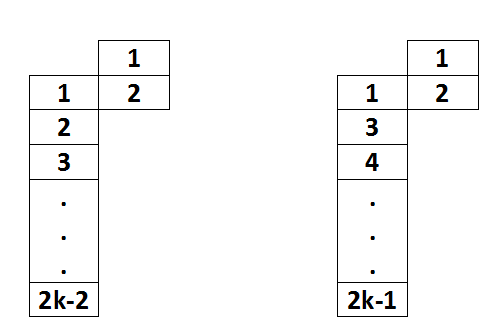
\includegraphics[width=4cm]{littlewood.png}.
\end{center}
The tableau on the left has weight $(2,2,1,\dots,1)$ with $|(2,2,1,\dots,1)|=2k\geq 6$. The partition $\gamma=(k-1,1)$ satisfies the conditions $(2\gamma)^{T}=(2,2,1,\dots,1)$, $|\gamma|=k$. However, for the tableau on the right there is no partition $\gamma$ satisfying $(2\gamma)^{T}=(2,1,\dots,1)$, $|\gamma|=k$ as the number of boxes in the first column of the Young diagram corresponding to the partition $(2,1, \dots,1)$ is odd (being equal to $2k-1$). 
\\Therefore, $\Sigma_{|\gamma|=k}N^{\lambda}_{(1),(2\gamma)^{T}}=N^{(2,2,1,\dots,1)}_{(1),(2,2,1,\dots,1)}$ and
$$\overline{soc}^{k+1}\Gamma_{\lambda}\cong(\Sigma_{|\gamma|=k}N^{\lambda}_{(1),(2\gamma)^{T}})\Gamma_{\langle\mu\rangle}$$
$$=N^{(2,2,1,\dots,1)}_{(1),(2,2,1\dots,1)}\Gamma_{\langle(1)\rangle}=\Gamma_{\langle(1)\rangle}.$$
This shows that the top layer of the socle filtration of $\Gamma_{\lambda}$ is a simple module.
\\We now show that the second top layer of $\Gamma_{\lambda}$ contains a submodule with multiplicity $n\ge 2$. According to Theorem 3.4,
$$\overline{soc}^{k}\Gamma_{\lambda}\cong \bigoplus_{|\mu|=|\lambda|-|2\gamma|}(\Sigma_{|\gamma|=k-1}N^{\lambda}_{\mu,(2\gamma)^{T}})\Gamma_{\langle\mu\rangle}.$$

It follows that $|\mu|=|\lambda|-|2\gamma|=3$. Therefore,
$$\overline{soc}^{k}\Gamma_{\lambda}\cong (\Sigma_{|\gamma|=k-1}N^{\lambda}_{(2,1),(2\gamma)^{T}})\Gamma_{\langle(2,1)\rangle}\oplus(\Sigma_{|\gamma|=k-1}N^{\lambda}_{(1,1,1),(2\gamma)^{T}})\Gamma_{\langle(1,1,1)\rangle}.$$
Consider the partition $\mu=(1,1,1).$ Explicit computations show that
$$\Sigma_{|\gamma|=k-1}N^{\lambda}_{(1,1,1),(2\gamma)^{T}}=2.$$ Indeed, there are two Littlewood-Richardson tableaux of shape $(2,2,1,\dots,1)/(1,1,1)$ 
\begin{center}

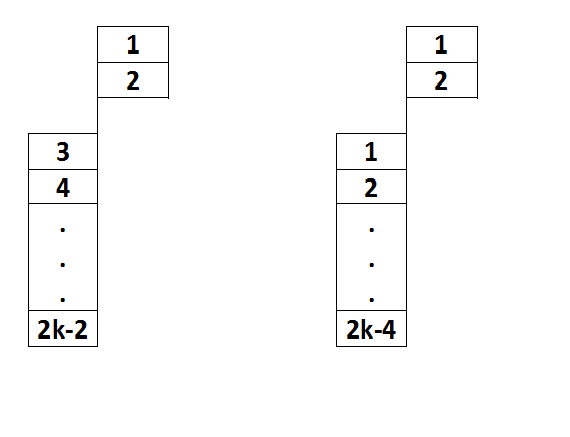
\includegraphics[width=5cm]{littlewood3.png}
\end{center}
(here we use that $d>5$).
The tableau on the left has weight $(1,1,\dots,1)=(2\gamma)^{T}$ for $\gamma=(k-1)$. For the right tableau the corresponding partition is $\gamma=(k-2,1)$. 

Therefore, in case $d$ is odd, Proposition 4.2 applies to $\Gamma_{(2,2,1,\dots,1)}$ and shows that $\Gamma_{(2,2,1,\dots,1)}$ is non-rigid.
\\
\textbf{Case 2} If $d=2k\geq6$, then $l=k+1$. From Theorem 3.4 we obtain 
$$\overline{soc}^{k+1}\Gamma_{\lambda}\cong \bigoplus_{|\mu|=|\lambda|-|2\gamma|}(\Sigma_{|\gamma|=k}N^{\lambda}_{\mu,(2\gamma)^{T}})\Gamma_{\langle\mu\rangle}.$$
Then we have $|\mu|=|\lambda|-|2\gamma|=0$, which makes this case easier. Therefore, the top layer of the socle filtration of $\Gamma_{(2,2,1,\dots,1)}$ is $\Gamma_{\langle(0)\rangle}$. 
In order to prove that the layer second from the top contains a submodule with multiplicity $n\ge 2$, we observe that 

$$\overline{soc}^{k}\Gamma_{\lambda}\cong \bigoplus_{|\mu|=|\lambda|-|2\gamma|}(\Sigma_{|\gamma|=k-1}N^{\lambda}_{\mu,(2\gamma)^{T}})\Gamma_{\langle\mu\rangle}$$

implies $|\mu|=|\lambda|-|(2\gamma)^{T}|=2$. Hence 
$$\overline{soc}^{k}\Gamma_{\lambda}\cong (\Sigma_{|\gamma|=k-1}N^{\lambda}_{(2),(2\gamma)^{T}})\Gamma_{\langle(2)\rangle}\oplus(\Sigma_{|\gamma|=k-1}N^{\lambda}_{(1,1),(2\gamma)^{T}})\Gamma_{\langle(1,1)\rangle}.$$
Consider the partition $(1,1)$. There are two Littlewood-Richardson tableaux of shape $(2,2,1,\dots,1)/(1,1)$ whose weights $\gamma$ satisfy $|(2\gamma)^{T}|=2k-2$
\begin{center}

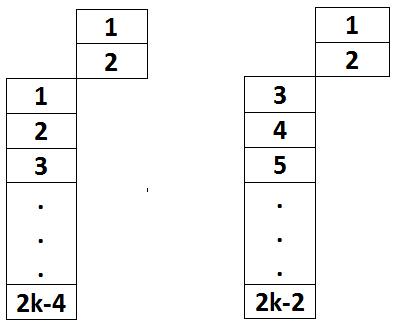
\includegraphics[width=3.5cm]{lit.png}
\end{center}
(here we use that $2k-4\geq 2$).
Therefore, $\Sigma_{|\gamma|=k-1}N^{\lambda}_{(1,1),(2\gamma)^{T}}=2$, which implies that, for even $d$, $\Gamma_{\langle(2,2,1,\dots,1)\rangle} $
is also non-rigid by Proposition 4.2.
\\Since $\Gamma_{\langle (2,2,1,\dots,1)\rangle}$ is non-rigid for $d\geq 6$, we have proven that  for any $d\geq 6$ the tensor representation $V^{\otimes d}$ of $\mathfrak{sp}_{\infty}$ contains at least one non-rigid indecomposable direct summand. $\blacksquare$

\section{Conclusion and open questions}
We have proven that all tensor representations $V^{\otimes d}$ of the simple finitary Lie algebra $\mathfrak{sp}_{\infty}$ contain at least one non-rigid indecomposable direct summand for $d\ge6$. Corollary 6.11 from \cite{cohen} states that the category of  tensor representations of $\mathfrak{sp}_{\infty}$  is equivalent to the category of tensor representations of $\mathfrak{so}_{\infty}$. Therefore, our results also apply to the tensor represenations of $\mathfrak{so}_{\infty}$. 
\\\\Along with Phillip Weiss' bachelor thesis, "Non-rigidity of tensor representations of $\mathfrak{gl}_{\infty}$" we have answered the question whether all indecomposable injective tensor modules are rigid for the simple finitary Lie algebras $\mathfrak{sl}_{\infty}$, $\mathfrak{sp}_{\infty}$ and $\mathfrak{so}_{\infty}$. However, we have not shown how many non-rigid indecomposable direct summands are contained in the decomposition of $V^{\otimes d}$ for $\mathfrak{sp}_{\infty}$. This is closely related to the general problem of computing the radical filtrations of the indecomposable direct summands of the $\mathfrak{sp}_{\infty}$-modules $V^{\otimes d}$ for $d\geq 6$, which could be an interesting avenue for further research.
\section{Appendix}
In this appendix one can find the results of our computations. The diagrams below represent the socle filtrations of indecomposable direct summands of $V^{\otimes d}$ for $d\leq10$. More precisely, each tower in these diagrams represents an indecomposable direct summand
of the corresponding tensor representation $V^{\otimes d}.$ The rows represent the socle
layers of the indecomposable submodule, with the bottom row representing the socle itself.

The computations below are done by \textbf{D. Harambas}; a correction of the original computations.

Layers of the socle filtration of the injective $\mathfrak{sp}_\infty-$modules $\Gamma_{\lambda}$ with $|\lambda| = $ 1 : \\\\
\begin{minipage}{1\textwidth}
\centering
\begin{tabular}{|c|}\hline
$\Gamma_{<(
1
)>}$
\\
\hline\end{tabular}\end{minipage}
\\



\bigskip
Layers of the socle filtration of the injective $\mathfrak{sp}_\infty-$modules $\Gamma_{\lambda}$ with $|\lambda| = $ 2 : \\\\
\begin{minipage}{.5\textwidth}
\centering
\begin{tabular}{|c|}\hline
$\Gamma_{<(
2
)>}$
\\
\hline\end{tabular}\end{minipage}
\begin{minipage}{.5\textwidth}
\centering
\begin{tabular}{|c|}\hline
$\Gamma_\emptyset$
\\ \hline
$\Gamma_{<(
1 , 
1
)>}$
\\
\hline\end{tabular}\end{minipage}
\\




\bigskip
Layers of the socle filtration of the injective $\mathfrak{sp}_\infty-$modules $\Gamma_{\lambda}$ with $|\lambda| = $ 3 : \\\\
\begin{minipage}{.33\textwidth}
\centering
\begin{tabular}{|c|}\hline
$\Gamma_{<(
3
)>}$
\\
\hline\end{tabular}\end{minipage}
\begin{minipage}{.33\textwidth}
\centering
\begin{tabular}{|c|}\hline
$\Gamma_{<(
1
)>}$
\\ \hline
$\Gamma_{<(
2 , 
1
)>}$
\\
\hline\end{tabular}\end{minipage}
\begin{minipage}{.33\textwidth}
\centering
\begin{tabular}{|c|}\hline
$\Gamma_{<(
1
)>}$
\\ \hline
$\Gamma_{<(
1 , 
1 , 
1
)>}$
\\
\hline\end{tabular}\end{minipage}
\\



\bigskip
Layers of the socle filtration of the injective $\mathfrak{sp}_\infty-$modules $\Gamma_{\lambda}$ with $|\lambda| = $ 4 : \\\\
\begin{minipage}{.2\textwidth}
\centering
\begin{tabular}{|c|}\hline
$\Gamma_{<(
4
)>}$
\\
\hline\end{tabular}\end{minipage}
\begin{minipage}{.2\textwidth}
\centering
\begin{tabular}{|c|}\hline
$\Gamma_{<(
2
)>}$
\\ \hline
$\Gamma_{<(
3 , 
1
)>}$
\\
\hline\end{tabular}\end{minipage}
\begin{minipage}{.2\textwidth}
\centering
\begin{tabular}{|c|}\hline
$\Gamma_\emptyset$
\\ \hline
$\Gamma_{<(
1 , 
1
)>}$
\\ \hline
$\Gamma_{<(
2 , 
2
)>}$
\\
\hline\end{tabular}\end{minipage}
\begin{minipage}{.2\textwidth}
\centering
\begin{tabular}{|c|}\hline
$\Gamma_{<(
2
)>} \oplus$
$\Gamma_{<(
1 , 
1
)>}$
\\ \hline
$\Gamma_{<(
2 , 
1 , 
1
)>}$
\\
\hline\end{tabular}\end{minipage}
\begin{minipage}{.2\textwidth}
\centering
\begin{tabular}{|c|}\hline
$\Gamma_\emptyset$
\\ \hline
$\Gamma_{<(
1 , 
1
)>}$
\\ \hline
$\Gamma_{<(
1 , 
1 , 
1 , 
1
)>}$
\\
\hline\end{tabular}\end{minipage}
\\



\bigskip
Layers of the socle filtration of the injective $\mathfrak{sp}_\infty-$modules $\Gamma_{\lambda}$ with $|\lambda| = $ 5 : \\\\
\begin{minipage}{.25\textwidth}
\centering
\begin{tabular}{|c|}\hline
$\Gamma_{<(
5
)>}$
\\
\hline\end{tabular}\end{minipage}
\begin{minipage}{.25\textwidth}
\centering
\begin{tabular}{|c|}\hline
$\Gamma_{<(
3
)>}$
\\ \hline
$\Gamma_{<(
4 , 
1
)>}$
\\
\hline\end{tabular}\end{minipage}
\begin{minipage}{.25\textwidth}
\centering
\begin{tabular}{|c|}\hline
$\Gamma_{<(
1
)>}$
\\ \hline
$\Gamma_{<(
2 , 
1
)>}$
\\ \hline
$\Gamma_{<(
3 , 
2
)>}$
\\
\hline\end{tabular}\end{minipage}
\begin{minipage}{.25\textwidth}
\centering
\begin{tabular}{|c|}\hline
$\Gamma_{<(
3
)>} \oplus$
$\Gamma_{<(
2 , 
1
)>}$
\\ \hline
$\Gamma_{<(
3 , 
1 , 
1
)>}$
\\
\hline\end{tabular}\end{minipage}
\bigskip
\begin{minipage}{.33\textwidth}
\centering
\begin{tabular}{|c|}\hline
$\Gamma_{<(
1
)>}$
\\ \hline
$\Gamma_{<(
2 , 
1
)>} \oplus$
$\Gamma_{<(
1 , 
1 , 
1
)>}$
\\ \hline
$\Gamma_{<(
2 , 
2 , 
1
)>}$
\\
\hline\end{tabular}\end{minipage}
\begin{minipage}{.33\textwidth}
\centering
\begin{tabular}{|c|}\hline
$\Gamma_{<(
1
)>}$
\\ \hline
$\Gamma_{<(
2 , 
1
)>} \oplus$
$\Gamma_{<(
1 , 
1 , 
1
)>}$
\\ \hline
$\Gamma_{<(
2 , 
1 , 
1 , 
1
)>}$
\\
\hline\end{tabular}\end{minipage}
\begin{minipage}{.33\textwidth}
\centering
\begin{tabular}{|c|}\hline
$\Gamma_{<(
1
)>}$
\\ \hline
$\Gamma_{<(
1 , 
1 , 
1
)>}$
\\ \hline
$\Gamma_{<(
1 , 
1 , 
1 , 
1 , 
1
)>}$
\\
\hline\end{tabular}\end{minipage}
\\




\bigskip
Layers of the socle filtration of the injective $\mathfrak{sp}_\infty-$modules $\Gamma_{\lambda}$ with $|\lambda| = $ 6 : \\\\
\begin{minipage}{.2\textwidth}
\centering
\begin{tabular}{|c|}\hline
$\Gamma_{<(
6
)>}$
\\
\hline\end{tabular}\end{minipage}
\begin{minipage}{.2\textwidth}
\centering
\begin{tabular}{|c|}\hline
$\Gamma_{<(
4
)>}$
\\ \hline
$\Gamma_{<(
5 , 
1
)>}$
\\
\hline\end{tabular}\end{minipage}
\begin{minipage}{.2\textwidth}
\centering
\begin{tabular}{|c|}\hline
$\Gamma_{<(
2
)>}$
\\ \hline
$\Gamma_{<(
3 , 
1
)>}$
\\ \hline
$\Gamma_{<(
4 , 
2
)>}$
\\
\hline\end{tabular}\end{minipage}
\begin{minipage}{.6\textwidth}
\centering
\begin{tabular}{|c|}\hline
$\Gamma_{<(
4
)>} \oplus$
$\Gamma_{<(
3 , 
1
)>}$
\\ \hline
$\Gamma_{<(
4 , 
1 , 
1
)>}$
\\
\hline\end{tabular}\end{minipage}
\bigskip
\begin{minipage}{.3\textwidth}
\centering
\begin{tabular}{|c|}\hline
$\Gamma_\emptyset$
\\ \hline
$\Gamma_{<(
1 , 
1
)>}$
\\ \hline
$\Gamma_{<(
2 , 
2
)>}$
\\ \hline
$\Gamma_{<(
3 , 
3
)>}$
\\
\hline\end{tabular}\end{minipage}
\begin{minipage}{.5\textwidth}
\centering
\begin{tabular}{|c|}\hline
$\Gamma_{<(
2
)>} \oplus$
$\Gamma_{<(
1 , 
1
)>}$
\\ \hline
$\Gamma_{<(
3 , 
1
)>} \oplus$
$\Gamma_{<(
2 , 
2
)>} \oplus$
$\Gamma_{<(
2 , 
1 , 
1
)>}$
\\ \hline
$\Gamma_{<(
3 , 
2 , 
1
)>}$
\\
\hline\end{tabular}\end{minipage}
\begin{minipage}{.3\textwidth}
\centering
\begin{tabular}{|c|}\hline
$\Gamma_{<(
2
)>}$
\\ \hline
$\Gamma_{<(
3 , 
1
)>} \oplus$
$\Gamma_{<(
2 , 
1 , 
1
)>}$
\\ \hline
$\Gamma_{<(
3 , 
1 , 
1 , 
1
)>}$
\\
\hline\end{tabular}\end{minipage}
\bigskip
\begin{minipage}{.15\textwidth}
\centering
\begin{tabular}{|c|}\hline
$\Gamma_{<(
2
)>}$
\\ \hline
$\Gamma_{<(
2 , 
1 , 
1
)>}$
\\ \hline
$\Gamma_{<(
2 , 
2 , 
2
)>}$
\\
\hline\end{tabular}\end{minipage}
\begin{minipage}{.35\textwidth}
\centering
\begin{tabular}{|c|}\hline
$\Gamma_\emptyset$
\\ \hline
$ 2 \Gamma_{<(
1 , 
1
)>}$
\\ \hline
$\Gamma_{<(
2 , 
2
)>} \oplus$
$\Gamma_{<(
2 , 
1 , 
1
)>} \oplus$
$\Gamma_{<(
1 , 
1 , 
1 , 
1
)>}$
\\ \hline
$\Gamma_{<(
2 , 
2 , 
1 , 
1
)>}$
\\
\hline\end{tabular}\end{minipage}
\begin{minipage}{.4\textwidth}
\centering
\begin{tabular}{|c|}\hline
$\Gamma_{<(
2
)>} \oplus$
$\Gamma_{<(
1 , 
1
)>}$
\\ \hline
$\Gamma_{<(
2 , 
1 , 
1
)>} \oplus$
$\Gamma_{<(
1 , 
1 , 
1 , 
1
)>}$
\\ \hline
$\Gamma_{<(
2 , 
1 , 
1 , 
1 , 
1
)>}$
\\
\hline\end{tabular}\end{minipage}
\begin{minipage}{.2\textwidth}
\centering
\begin{tabular}{|c|}\hline
$\Gamma_\emptyset$
\\ \hline
$\Gamma_{<(
1 , 
1
)>}$
\\ \hline
$\Gamma_{<(
1 , 
1 , 
1 , 
1
)>}$
\\ \hline
$\Gamma_{<(
1 , 
1 , 
1 , 
1 , 
1 , 
1
)>}$
\\
\hline\end{tabular}\end{minipage}
\\




\bigskip
Layers of the socle filtration of the injective $\mathfrak{sp}_\infty-$modules $\Gamma_{\lambda}$ with $|\lambda| = $ 7 : \\\\
\begin{minipage}{.2\textwidth}
\centering
\begin{tabular}{|c|}\hline
$\Gamma_{<(
7
)>}$
\\
\hline\end{tabular}\end{minipage}
\begin{minipage}{.2\textwidth}
\centering
\begin{tabular}{|c|}\hline
$\Gamma_{<(
5
)>}$
\\ \hline
$\Gamma_{<(
6 , 
1
)>}$
\\
\hline\end{tabular}\end{minipage}
\begin{minipage}{.2\textwidth}
\centering
\begin{tabular}{|c|}\hline
$\Gamma_{<(
3
)>}$
\\ \hline
$\Gamma_{<(
4 , 
1
)>}$
\\ \hline
$\Gamma_{<(
5 , 
2
)>}$
\\
\hline\end{tabular}\end{minipage}
\begin{minipage}{.2\textwidth}
\centering
\begin{tabular}{|c|}\hline
$\Gamma_{<(
5
)>} \oplus$
$\Gamma_{<(
4 , 
1
)>}$
\\ \hline
$\Gamma_{<(
5 , 
1 , 
1
)>}$
\\
\hline\end{tabular}\end{minipage}
\begin{minipage}{.2\textwidth}
\centering
\begin{tabular}{|c|}\hline
$\Gamma_{<(
1
)>}$
\\ \hline
$\Gamma_{<(
2 , 
1
)>}$
\\ \hline
$\Gamma_{<(
3 , 
2
)>}$
\\ \hline
$\Gamma_{<(
4 , 
3
)>}$
\\
\hline\end{tabular}\end{minipage}
\bigskip
\begin{minipage}{.4\textwidth}
\centering
\begin{tabular}{|c|}\hline
$\Gamma_{<(
3
)>} \oplus$
$\Gamma_{<(
2 , 
1
)>}$
\\ \hline
$\Gamma_{<(
4 , 
1
)>} \oplus$
$\Gamma_{<(
3 , 
2
)>} \oplus$
$\Gamma_{<(
3 , 
1 , 
1
)>}$
\\ \hline
$\Gamma_{<(
4 , 
2 , 
1
)>}$
\\
\hline\end{tabular}\end{minipage}
\begin{minipage}{.3\textwidth}
\centering
\begin{tabular}{|c|}\hline
$\Gamma_{<(
3
)>}$
\\ \hline
$\Gamma_{<(
4 , 
1
)>} \oplus$
$\Gamma_{<(
3 , 
1 , 
1
)>}$
\\ \hline
$\Gamma_{<(
4 , 
1 , 
1 , 
1
)>}$
\\
\hline\end{tabular}\end{minipage}
\begin{minipage}{.3\textwidth}
\centering
\begin{tabular}{|c|}\hline
$\Gamma_{<(
1
)>}$
\\ \hline
$\Gamma_{<(
2 , 
1
)>} \oplus$
$\Gamma_{<(
1 , 
1 , 
1
)>}$
\\ \hline
$\Gamma_{<(
3 , 
2
)>} \oplus$
$\Gamma_{<(
2 , 
2 , 
1
)>}$
\\ \hline
$\Gamma_{<(
3 , 
3 , 
1
)>}$
\\
\hline\end{tabular}\end{minipage}
\bigskip
\begin{minipage}{.25\textwidth}
\centering
\begin{tabular}{|c|}\hline
$\Gamma_{<(
3
)>} \oplus$
$\Gamma_{<(
2 , 
1
)>}$
\\ \hline
$\Gamma_{<(
3 , 
1 , 
1
)>} \oplus$
$\Gamma_{<(
2 , 
2 , 
1
)>}$
\\ \hline
$\Gamma_{<(
3 , 
2 , 
2
)>}$
\\
\hline\end{tabular}\end{minipage}
\begin{minipage}{.6\textwidth}
\centering
\begin{tabular}{|c|}\hline
$\Gamma_{<(
1
)>}$
\\ \hline
$ 2 \Gamma_{<(
2 , 
1
)>} \oplus$
$\Gamma_{<(
1 , 
1 , 
1
)>}$
\\ \hline
$\Gamma_{<(
3 , 
2
)>} \oplus$
$\Gamma_{<(
3 , 
1 , 
1
)>} \oplus$
$\Gamma_{<(
2 , 
2 , 
1
)>} \oplus$
$\Gamma_{<(
2 , 
1 , 
1 , 
1
)>}$
\\ \hline
$\Gamma_{<(
3 , 
2 , 
1 , 
1
)>}$
\\
\hline\end{tabular}\end{minipage}
\begin{minipage}{.3\textwidth}
\centering
\begin{tabular}{|c|}\hline
$\Gamma_{<(
3
)>} \oplus$
$\Gamma_{<(
2 , 
1
)>}$
\\ \hline
$\Gamma_{<(
3 , 
1 , 
1
)>} \oplus$
$\Gamma_{<(
2 , 
1 , 
1 , 
1
)>}$
\\ \hline
$\Gamma_{<(
3 , 
1 , 
1 , 
1 , 
1
)>}$
\\
\hline\end{tabular}\end{minipage}
\bigskip
\begin{minipage}{.3\textwidth}
\centering
\begin{tabular}{|c|}\hline
$\Gamma_{<(
1
)>}$
\\ \hline
$\Gamma_{<(
1 , 
1 , 
1
)>} \oplus$
$\Gamma_{<(
2 , 
1
)>}$
\\ \hline
$\Gamma_{<(
2 , 
2 , 
1
)>} \oplus$
$\Gamma_{<(
2 , 
1 , 
1 , 
1
)>}$
\\ \hline
$\Gamma_{<(
2 , 
2 , 
2 , 
1
)>}$
\\
\hline\end{tabular}\end{minipage}
\begin{minipage}{.5\textwidth}
\centering
\begin{tabular}{|c|}\hline
$\Gamma_{<(
1
)>}$
\\ \hline
$\Gamma_{<(
2 , 
1
)>} \oplus$
$ 2 \Gamma_{<(
1 , 
1 , 
1
)>}$
\\ \hline
$\Gamma_{<(
2 , 
2 , 
1
)>} \oplus$
$\Gamma_{<(
2 , 
1 , 
1 , 
1
)>} \oplus$
$\Gamma_{<(
1 , 
1 , 
1 , 
1 , 
1
)>}$
\\ \hline
$\Gamma_{<(
2 , 
2 , 
1 , 
1 , 
1
)>}$
\\
\hline\end{tabular}\end{minipage}
\begin{minipage}{.3\textwidth}
\centering
\begin{tabular}{|c|}\hline
$\Gamma_{<(
1
)>}$
\\ \hline
$\Gamma_{<(
2 , 
1
)>} \oplus$
$\Gamma_{<(
1 , 
1 , 
1
)>}$
\\ \hline
$\Gamma_{<(
2 , 
1 , 
1 , 
1
)>} \oplus$
$\Gamma_{<(
1 , 
1 , 
1 , 
1 , 
1
)>}$
\\ \hline
$\Gamma_{<(
2 , 
1 , 
1 , 
1 , 
1 , 
1
)>}$
\\
\hline\end{tabular}\end{minipage}
\begin{minipage}{1\textwidth}
\centering
\begin{tabular}{|c|}\hline
$\Gamma_{<(
1
)>}$
\\ \hline
$\Gamma_{<(
1 , 
1 , 
1
)>}$
\\ \hline
$\Gamma_{<(
1 , 
1 , 
1 , 
1 , 
1
)>}$
\\ \hline
$\Gamma_{<(
1 , 
1 , 
1 , 
1 , 
1 , 
1 , 
1
)>}$
\\
\hline\end{tabular}\end{minipage}
\\




\bigskip
Layers of the socle filtration of the injective $\mathfrak{sp}_\infty-$modules $\Gamma_{\lambda}$ with $|\lambda| = $ 8 : \\\\
\begin{minipage}{.2\textwidth}
\centering
\begin{tabular}{|c|}\hline
$\Gamma_{<(
8
)>}$
\\
\hline\end{tabular}\end{minipage}
\begin{minipage}{.2\textwidth}
\centering
\begin{tabular}{|c|}\hline
$\Gamma_{<(
6
)>}$
\\ \hline
$\Gamma_{<(
7 , 
1
)>}$
\\
\hline\end{tabular}\end{minipage}
\begin{minipage}{.2\textwidth}
\centering
\begin{tabular}{|c|}\hline
$\Gamma_{<(
4
)>}$
\\ \hline
$\Gamma_{<(
5 , 
1
)>}$
\\ \hline
$\Gamma_{<(
6 , 
2
)>}$
\\
\hline\end{tabular}\end{minipage}
\begin{minipage}{.2\textwidth}
\centering
\begin{tabular}{|c|}\hline
$\Gamma_{<(
6
)>} \oplus$
$\Gamma_{<(
5 , 
1
)>}$
\\ \hline
$\Gamma_{<(
6 , 
1 , 
1
)>}$
\\
\hline\end{tabular}\end{minipage}
\begin{minipage}{.2\textwidth}
\centering
\begin{tabular}{|c|}\hline
$\Gamma_{<(
2
)>}$
\\ \hline
$\Gamma_{<(
3 , 
1
)>}$
\\ \hline
$\Gamma_{<(
4 , 
2
)>}$
\\ \hline
$\Gamma_{<(
5 , 
3
)>}$
\\
\hline\end{tabular}\end{minipage}
\bigskip
\begin{minipage}{.4\textwidth}
\centering
\begin{tabular}{|c|}\hline
$\Gamma_{<(
4
)>} \oplus$
$\Gamma_{<(
3 , 
1
)>}$
\\ \hline
$\Gamma_{<(
5 , 
1
)>} \oplus$
$\Gamma_{<(
4 , 
2
)>} \oplus$
$\Gamma_{<(
4 , 
1 , 
1
)>}$
\\ \hline
$\Gamma_{<(
5 , 
2 , 
1
)>}$
\\
\hline\end{tabular}\end{minipage}
\begin{minipage}{.4\textwidth}
\centering
\begin{tabular}{|c|}\hline
$\Gamma_{<(
4
)>}$
\\ \hline
$\Gamma_{<(
5 , 
1
)>} \oplus$
$\Gamma_{<(
4 , 
1 , 
1
)>}$
\\ \hline
$\Gamma_{<(
5 , 
1 , 
1 , 
1
)>}$
\\
\hline\end{tabular}\end{minipage}
\begin{minipage}{.2\textwidth}
\centering
\begin{tabular}{|c|}\hline
$\Gamma_\emptyset$
\\ \hline
$\Gamma_{<(
1 , 
1
)>}$
\\ \hline
$\Gamma_{<(
2 , 
2
)>}$
\\ \hline
$\Gamma_{<(
3 , 
3
)>}$
\\ \hline
$\Gamma_{<(
4 , 
4
)>}$
\\
\hline\end{tabular}\end{minipage}
\bigskip
\begin{minipage}{.5\textwidth}
\centering
\begin{tabular}{|c|}\hline
$\Gamma_{<(
2
)>} \oplus$
$\Gamma_{<(
1 , 
1
)>}$
\\ \hline
$\Gamma_{<(
3 , 
1
)>} \oplus$
$\Gamma_{<(
2 , 
2
)>} \oplus$
$\Gamma_{<(
2 , 
1 , 
1
)>}$
\\ \hline
$\Gamma_{<(
4 , 
2
)>} \oplus$
$\Gamma_{<(
3 , 
3
)>} \oplus$
$\Gamma_{<(
3 , 
2 , 
1
)>}$
\\ \hline
$\Gamma_{<(
4 , 
3 , 
1
)>}$
\\
\hline\end{tabular}\end{minipage}
\begin{minipage}{.5\textwidth}
\centering
\begin{tabular}{|c|}\hline
$\Gamma_{<(
4
)>} \oplus$
$\Gamma_{<(
3 , 
1
)>} \oplus$
$\Gamma_{<(
2 , 
2
)>}$
\\ \hline
$\Gamma_{<(
4 , 
1 , 
1
)>} \oplus$
$\Gamma_{<(
3 , 
2 , 
1
)>}$
\\ \hline
$\Gamma_{<(
4 , 
2 , 
2
)>}$
\\
\hline\end{tabular}\end{minipage}
\bigskip
\begin{minipage}{.5\textwidth}
\centering
\begin{tabular}{|c|}\hline
$\Gamma_{<(
2
)>}$
\\ \hline
$ 2 \Gamma_{<(
3 , 
1
)>} \oplus$
$\Gamma_{<(
2 , 
1 , 
1
)>}$
\\ \hline
$\Gamma_{<(
4 , 
2
)>} \oplus$
$\Gamma_{<(
4 , 
1 , 
1
)>} \oplus$
$\Gamma_{<(
3 , 
2 , 
1
)>} \oplus$
$\Gamma_{<(
3 , 
1 , 
1 , 
1
)>}$
\\ \hline
$\Gamma_{<(
4 , 
2 , 
1 , 
1
)>}$
\\
\hline\end{tabular}\end{minipage}
\begin{minipage}{.28\textwidth}
\centering
\begin{tabular}{|c|}\hline
$\Gamma_{<(
4
)>} \oplus$
$\Gamma_{<(
3 , 
1
)>}$
\\ \hline
$\Gamma_{<(
4 , 
1 , 
1
)>} \oplus$
$\Gamma_{<(
3 , 
1 , 
1 , 
1
)>}$
\\ \hline
$\Gamma_{<(
4 , 
1 , 
1 , 
1 , 
1
)>}$
\\
\hline\end{tabular}\end{minipage}
\begin{minipage}{.26\textwidth}
\centering
\begin{tabular}{|c|}\hline
$\Gamma_{<(
2
)>}$
\\ \hline
$\Gamma_{<(
3 , 
1
)>} \oplus$
$\Gamma_{<(
2 , 
1 , 
1
)>}$
\\ \hline
$\Gamma_{<(
3 , 
2 , 
1
)>} \oplus$
$\Gamma_{<(
2 , 
2 , 
2
)>}$
\\ \hline
$\Gamma_{<(
3 , 
3 , 
2
)>}$
\\
\hline\end{tabular}\end{minipage}
\bigskip
\begin{minipage}{.4\textwidth}
\centering
\begin{tabular}{|c|}\hline
$\Gamma_\emptyset$
\\ \hline
$ 2 \Gamma_{<(
1 , 
1
)>}$
\\ \hline
$ 2 \Gamma_{<(
2 , 
2
)>} \oplus$
$\Gamma_{<(
2 , 
1 , 
1
)>} \oplus$
$\Gamma_{<(
1 , 
1 , 
1 , 
1
)>}$
\\ \hline
$\Gamma_{<(
3 , 
3
)>} \oplus$
$\Gamma_{<(
3 , 
2 , 
1
)>} \oplus$
$\Gamma_{<(
2 , 
2 , 
1 , 
1
)>}$
\\ \hline
$\Gamma_{<(
3 , 
3 , 
1 , 
1
)>}$
\\
\hline\end{tabular}\end{minipage}
\begin{minipage}{.6\textwidth}
\centering
\begin{tabular}{|c|}\hline
$\Gamma_{<(
2
)>} \oplus$
$\Gamma_{<(
1 , 
1
)>}$
\\ \hline
$ 2 \Gamma_{<(
2 , 
1 , 
1
)>} \oplus$
$\Gamma_{<(
3 , 
1
)>} \oplus$
$\Gamma_{<(
2 , 
2
)>}$
\\ \hline
$\Gamma_{<(
3 , 
2 , 
1
)>} \oplus$
$\Gamma_{<(
3 , 
1 , 
1 , 
1
)>} \oplus$
$\Gamma_{<(
2 , 
2 , 
2
)>} \oplus$
$\Gamma_{<(
2 , 
2 , 
1 , 
1
)>}$
\\ \hline
$\Gamma_{<(
3 , 
2 , 
2 , 
1
)>}$
\\
\hline\end{tabular}\end{minipage}
\bigskip
\begin{minipage}{.6\textwidth}
\centering
\begin{tabular}{|c|}\hline
$\Gamma_{<(
2
)>} \oplus$
$\Gamma_{<(
1 , 
1
)>}$
\\ \hline
$\Gamma_{<(
3 , 
1
)>} \oplus$
$\Gamma_{<(
2 , 
2
)>} \oplus$
$ 2 \Gamma_{<(
2 , 
1 , 
1
)>} \oplus$
$\Gamma_{<(
1 , 
1 , 
1 , 
1
)>}$
\\ \hline
$\Gamma_{<(
3 , 
2 , 
1
)>} \oplus$
$\Gamma_{<(
3 , 
1 , 
1 , 
1
)>} \oplus$
$\Gamma_{<(
2 , 
2 , 
1 , 
1
)>} \oplus$
$\Gamma_{<(
2 , 
1 , 
1 , 
1 , 
1
)>}$
\\ \hline
$\Gamma_{<(
3 , 
2 , 
1 , 
1 , 
1
)>}$
\\
\hline\end{tabular}\end{minipage}
\begin{minipage}{.4\textwidth}
\centering
\begin{tabular}{|c|}\hline
$\Gamma_{<(
2
)>}$
\\ \hline
$\Gamma_{<(
3 , 
1
)>} \oplus$
$\Gamma_{<(
2 , 
1 , 
1
)>}$
\\ \hline
$\Gamma_{<(
3 , 
1 , 
1 , 
1
)>} \oplus$
$\Gamma_{<(
2 , 
1 , 
1 , 
1 , 
1
)>}$
\\ \hline
$\Gamma_{<(
3 , 
1 , 
1 , 
1 , 
1 , 
1
)>}$
\\
\hline\end{tabular}\end{minipage}
\bigskip
\begin{minipage}{.4\textwidth}
\centering
\begin{tabular}{|c|}\hline
$\Gamma_\emptyset$
\\ \hline
$\Gamma_{<(
1 , 
1
)>}$
\\ \hline
$\Gamma_{<(
1 , 
1 , 
1 , 
1
)>} \oplus$
$\Gamma_{<(
2 , 
2
)>}$
\\ \hline
$\Gamma_{<(
2 , 
2 , 
1 , 
1
)>}$
\\ \hline
$\Gamma_{<(
2 , 
2 , 
2 , 
2
)>}$
\\
\hline\end{tabular}\end{minipage}
\begin{minipage}{.6\textwidth}
\centering
\begin{tabular}{|c|}\hline
$\Gamma_{<(
2
)>} \oplus$
$\Gamma_{<(
1 , 
1
)>}$
\\ \hline
$ 2 \Gamma_{<(
2 , 
1 , 
1
)>} \oplus$
$\Gamma_{<(
1 , 
1 , 
1 , 
1
)>}$
\\ \hline
$\Gamma_{<(
2 , 
2 , 
2
)>} \oplus$
$\Gamma_{<(
2 , 
2 , 
1 , 
1
)>} \oplus$
$\Gamma_{<(
2 , 
1 , 
1 , 
1 , 
1
)>}$
\\ \hline
$\Gamma_{<(
2 , 
2 , 
2 , 
1 , 
1
)>}$
\\
\hline\end{tabular}\end{minipage}
\bigskip
\begin{minipage}{.6\textwidth}
\centering
\begin{tabular}{|c|}\hline
$\Gamma_\emptyset$
\\ \hline
$ 2 \Gamma_{<(
1 , 
1
)>}$
\\ \hline
$\Gamma_{<(
2 , 
2
)>} \oplus$
$\Gamma_{<(
2 , 
1 , 
1
)>} \oplus$
$ 2 \Gamma_{<(
1 , 
1 , 
1 , 
1
)>}$
\\ \hline
$\Gamma_{<(
2 , 
2 , 
1 , 
1
)>} \oplus$
$\Gamma_{<(
2 , 
1 , 
1 , 
1 , 
1
)>} \oplus$
$\Gamma_{<(
1 , 
1 , 
1 , 
1 , 
1 , 
1
)>}$
\\ \hline
$\Gamma_{<(
2 , 
2 , 
1 , 
1 , 
1 , 
1
)>}$
\\
\hline\end{tabular}\end{minipage}
\begin{minipage}{.4\textwidth}
\centering
\begin{tabular}{|c|}\hline
$\Gamma_{<(
2
)>} \oplus$
$\Gamma_{<(
1 , 
1
)>}$
\\ \hline
$\Gamma_{<(
2 , 
1 , 
1
)>} \oplus$
$\Gamma_{<(
1 , 
1 , 
1 , 
1
)>}$
\\ \hline
$\Gamma_{<(
2 , 
1 , 
1 , 
1 , 
1
)>} \oplus$
$\Gamma_{<(
1 , 
1 , 
1 , 
1 , 
1 , 
1
)>}$
\\ \hline
$\Gamma_{<(
2 , 
1 , 
1 , 
1 , 
1 , 
1 , 
1
)>}$
\\
\hline\end{tabular}\end{minipage}
\bigskip
\begin{minipage}{1\textwidth}
\centering
\begin{tabular}{|c|}\hline
$\Gamma_\emptyset$
\\ \hline
$\Gamma_{<(
1 , 
1
)>}$
\\ \hline
$\Gamma_{<(
1 , 
1 , 
1 , 
1
)>}$
\\ \hline
$\Gamma_{<(
1 , 
1 , 
1 , 
1 , 
1 , 
1
)>}$
\\ \hline
$\Gamma_{<(
1 , 
1 , 
1 , 
1 , 
1 , 
1 , 
1 , 
1
)>}$
\\
\hline\end{tabular}\end{minipage}
\\




\bigskip
Layers of the socle filtration of the injective $\mathfrak{sp}_\infty-$modules $\Gamma_{\lambda}$ with $|\lambda| = $ 9 : \\\\
\begin{minipage}{.2\textwidth}
\centering
\begin{tabular}{|c|}\hline
$\Gamma_{<(
9
)>}$
\\
\hline\end{tabular}\end{minipage}
\begin{minipage}{.2\textwidth}
\centering
\begin{tabular}{|c|}\hline
$\Gamma_{<(
7
)>}$
\\ \hline
$\Gamma_{<(
8 , 
1
)>}$
\\
\hline\end{tabular}\end{minipage}
\begin{minipage}{.2\textwidth}
\centering
\begin{tabular}{|c|}\hline
$\Gamma_{<(
5
)>}$
\\ \hline
$\Gamma_{<(
6 , 
1
)>}$
\\ \hline
$\Gamma_{<(
7 , 
2
)>}$
\\
\hline\end{tabular}\end{minipage}
\begin{minipage}{.2\textwidth}
\centering
\begin{tabular}{|c|}\hline
$\Gamma_{<(
7
)>} \oplus$
$\Gamma_{<(
6 , 
1
)>}$
\\ \hline
$\Gamma_{<(
7 , 
1 , 
1
)>}$
\\
\hline\end{tabular}\end{minipage}
\begin{minipage}{.2\textwidth}
\centering
\begin{tabular}{|c|}\hline
$\Gamma_{<(
3
)>}$
\\ \hline
$\Gamma_{<(
4 , 
1
)>}$
\\ \hline
$\Gamma_{<(
5 , 
2
)>}$
\\ \hline
$\Gamma_{<(
6 , 
3
)>}$
\\
\hline\end{tabular}\end{minipage}
\bigskip
\begin{minipage}{.4\textwidth}
\centering
\begin{tabular}{|c|}\hline
$\Gamma_{<(
5
)>} \oplus$
$\Gamma_{<(
4 , 
1
)>}$
\\ \hline
$\Gamma_{<(
6 , 
1
)>} \oplus$
$\Gamma_{<(
5 , 
2
)>} \oplus$
$\Gamma_{<(
5 , 
1 , 
1
)>}$
\\ \hline
$\Gamma_{<(
6 , 
2 , 
1
)>}$
\\
\hline\end{tabular}\end{minipage}
\begin{minipage}{.3\textwidth}
\centering
\begin{tabular}{|c|}\hline
$\Gamma_{<(
5
)>}$
\\ \hline
$\Gamma_{<(
6 , 
1
)>} \oplus$
$\Gamma_{<(
5 , 
1 , 
1
)>}$
\\ \hline
$\Gamma_{<(
6 , 
1 , 
1 , 
1
)>}$
\\
\hline\end{tabular}\end{minipage}
\begin{minipage}{.3\textwidth}
\centering
\begin{tabular}{|c|}\hline
$\Gamma_{<(
1
)>}$
\\ \hline
$\Gamma_{<(
2 , 
1
)>}$
\\ \hline
$\Gamma_{<(
3 , 
2
)>}$
\\ \hline
$\Gamma_{<(
4 , 
3
)>}$
\\ \hline
$\Gamma_{<(
5 , 
4
)>}$
\\
\hline\end{tabular}\end{minipage}
\bigskip
\begin{minipage}{.5\textwidth}
\centering
\begin{tabular}{|c|}\hline
$\Gamma_{<(
3
)>} \oplus$
$\Gamma_{<(
2 , 
1
)>}$
\\ \hline
$\Gamma_{<(
4 , 
1
)>} \oplus$
$\Gamma_{<(
3 , 
2
)>} \oplus$
$\Gamma_{<(
3 , 
1 , 
1
)>}$
\\ \hline
$\Gamma_{<(
5 , 
2
)>} \oplus$
$\Gamma_{<(
4 , 
3
)>} \oplus$
$\Gamma_{<(
4 , 
2 , 
1
)>}$
\\ \hline
$\Gamma_{<(
5 , 
3 , 
1
)>}$
\\
\hline\end{tabular}\end{minipage}
\begin{minipage}{.5\textwidth}
\centering
\begin{tabular}{|c|}\hline
$\Gamma_{<(
5
)>} \oplus$
$\Gamma_{<(
4 , 
1
)>} \oplus$
$\Gamma_{<(
3 , 
2
)>}$
\\ \hline
$\Gamma_{<(
5 , 
1 , 
1
)>} \oplus$
$\Gamma_{<(
4 , 
2 , 
1
)>}$
\\ \hline
$\Gamma_{<(
5 , 
2 , 
2
)>}$
\\
\hline\end{tabular}\end{minipage}
\bigskip
\begin{minipage}{.6\textwidth}
\centering
\begin{tabular}{|c|}\hline
$\Gamma_{<(
3
)>}$
\\ \hline
$ 2 \Gamma_{<(
4 , 
1
)>} \oplus$
$\Gamma_{<(
3 , 
1 , 
1
)>}$
\\ \hline
$\Gamma_{<(
5 , 
2
)>} \oplus$
$\Gamma_{<(
5 , 
1 , 
1
)>} \oplus$
$\Gamma_{<(
4 , 
2 , 
1
)>} \oplus$
$\Gamma_{<(
4 , 
1 , 
1 , 
1
)>}$
\\ \hline
$\Gamma_{<(
5 , 
2 , 
1 , 
1
)>}$
\\
\hline\end{tabular}\end{minipage}
\begin{minipage}{.4\textwidth}
\centering
\begin{tabular}{|c|}\hline
$\Gamma_{<(
5
)>} \oplus$
$\Gamma_{<(
4 , 
1
)>}$
\\ \hline
$\Gamma_{<(
5 , 
1 , 
1
)>} \oplus$
$\Gamma_{<(
4 , 
1 , 
1 , 
1
)>}$
\\ \hline
$\Gamma_{<(
5 , 
1 , 
1 , 
1 , 
1
)>}$
\\
\hline\end{tabular}\end{minipage}
\bigskip
\begin{minipage}{.4\textwidth}
\centering
\begin{tabular}{|c|}\hline
$\Gamma_{<(
1
)>}$
\\ \hline
$\Gamma_{<(
2 , 
1
)>} \oplus$
$\Gamma_{<(
1 , 
1 , 
1
)>}$
\\ \hline
$\Gamma_{<(
3 , 
2
)>} \oplus$
$\Gamma_{<(
2 , 
2 , 
1
)>}$
\\ \hline
$\Gamma_{<(
4 , 
3
)>} \oplus$
$\Gamma_{<(
3 , 
3 , 
1
)>}$
\\ \hline
$\Gamma_{<(
4 , 
4 , 
1
)>}$
\\
\hline\end{tabular}\end{minipage}
\begin{minipage}{.6\textwidth}
\centering
\begin{tabular}{|c|}\hline
$\Gamma_{<(
3
)>} \oplus$
$\Gamma_{<(
2 , 
1
)>}$
\\ \hline
$\Gamma_{<(
4 , 
1
)>} \oplus$
$\Gamma_{<(
3 , 
2
)>} \oplus$
$\Gamma_{<(
3 , 
1 , 
1
)>} \oplus$
$\Gamma_{<(
2 , 
2 , 
1
)>}$
\\ \hline
$\Gamma_{<(
4 , 
2 , 
1
)>} \oplus$
$\Gamma_{<(
3 , 
3 , 
1
)>} \oplus$
$\Gamma_{<(
3 , 
2 , 
2
)>}$
\\ \hline
$\Gamma_{<(
4 , 
3 , 
2
)>}$
\\
\hline\end{tabular}\end{minipage}
\bigskip
\begin{minipage}{.5\textwidth}
\centering
\begin{tabular}{|c|}\hline
$\Gamma_{<(
1
)>}$
\\ \hline
$ 2 \Gamma_{<(
2 , 
1
)>} \oplus$
$\Gamma_{<(
1 , 
1 , 
1
)>}$
\\ \hline
$ 2 \Gamma_{<(
3 , 
2
)>} \oplus$
$\Gamma_{<(
3 , 
1 , 
1
)>} \oplus$
$\Gamma_{<(
2 , 
2 , 
1
)>} \oplus$
$\Gamma_{<(
2 , 
1 , 
1 , 
1
)>}$
\\ \hline
$\Gamma_{<(
4 , 
3
)>} \oplus$
$\Gamma_{<(
4 , 
2 , 
1
)>} \oplus$
$\Gamma_{<(
3 , 
3 , 
1
)>} \oplus$
$\Gamma_{<(
3 , 
2 , 
1 , 
1
)>}$
\\ \hline
$\Gamma_{<(
4 , 
3 , 
1 , 
1
)>}$
\\
\hline\end{tabular}\end{minipage}
\begin{minipage}{.6\textwidth}
\centering
\begin{tabular}{|c|}\hline
$\Gamma_{<(
3
)>} \oplus$
$\Gamma_{<(
2 , 
1
)>}$
\\ \hline
$ 2 \Gamma_{<(
3 , 
1 , 
1
)>} \oplus$
$\Gamma_{<(
4 , 
1
)>} \oplus$
$\Gamma_{<(
3 , 
2
)>} \oplus$
$\Gamma_{<(
2 , 
2 , 
1
)>}$
\\ \hline
$\Gamma_{<(
4 , 
2 , 
1
)>} \oplus$
$\Gamma_{<(
4 , 
1 , 
1 , 
1
)>} \oplus$
$\Gamma_{<(
3 , 
2 , 
2
)>} \oplus$
$\Gamma_{<(
3 , 
2 , 
1 , 
1
)>}$
\\ \hline
$\Gamma_{<(
4 , 
2 , 
2 , 
1
)>}$
\\
\hline\end{tabular}\end{minipage}
\bigskip
\begin{minipage}{.5\textwidth}
\centering
\begin{tabular}{|c|}\hline
$\Gamma_{<(
3
)>} \oplus$
$\Gamma_{<(
2 , 
1
)>}$
\\ \hline
$\Gamma_{<(
4 , 
1
)>} \oplus$
$\Gamma_{<(
3 , 
2
)>} \oplus$
$ 2 \Gamma_{<(
3 , 
1 , 
1
)>} \oplus$
$\Gamma_{<(
2 , 
1 , 
1 , 
1
)>}$
\\ \hline
$\Gamma_{<(
4 , 
2 , 
1
)>} \oplus$
$\Gamma_{<(
4 , 
1 , 
1 , 
1
)>} \oplus$
$\Gamma_{<(
3 , 
2 , 
1 , 
1
)>} \oplus$
$\Gamma_{<(
3 , 
1 , 
1 , 
1 , 
1
)>}$
\\ \hline
$\Gamma_{<(
4 , 
2 , 
1 , 
1 , 
1
)>}$
\\
\hline\end{tabular}\end{minipage}
\begin{minipage}{.57\textwidth}
\centering
\begin{tabular}{|c|}\hline
$\Gamma_{<(
3
)>}$
\\ \hline
$\Gamma_{<(
4 , 
1
)>} \oplus$
$\Gamma_{<(
3 , 
1 , 
1
)>}$
\\ \hline
$\Gamma_{<(
4 , 
1 , 
1 , 
1
)>} \oplus$
$\Gamma_{<(
3 , 
1 , 
1 , 
1 , 
1
)>}$
\\ \hline
$\Gamma_{<(
4 , 
1 , 
1 , 
1 , 
1 , 
1
)>}$
\\
\hline\end{tabular}\end{minipage}
\begin{minipage}{.123\textwidth}
\centering
\begin{tabular}{|c|}\hline
$\Gamma_{<(
3
)>}$
\\ \hline
$\Gamma_{<(
3 , 
1 , 
1
)>}$
\\ \hline
$\Gamma_{<(
3 , 
2 , 
2
)>}$
\\ \hline
$\Gamma_{<(
3 , 
3 , 
3
)>}$
\\
\hline\end{tabular}\end{minipage}
\bigskip
\begin{minipage}{.526\textwidth}
\centering
\begin{tabular}{|c|}\hline
$\Gamma_{<(
1
)>}$
\\ \hline
$ 2 \Gamma_{<(
2 , 
1
)>} \oplus$
$\Gamma_{<(
1 , 
1 , 
1
)>}$
\\ \hline
$ 2 \Gamma_{<(
2 , 
2 , 
1
)>} \oplus$
$\Gamma_{<(
3 , 
2
)>} \oplus$
$\Gamma_{<(
3 , 
1 , 
1
)>} \oplus$
$\Gamma_{<(
2 , 
1 , 
1 , 
1
)>}$
\\ \hline
$\Gamma_{<(
3 , 
3 , 
1
)>} \oplus$
$\Gamma_{<(
3 , 
2 , 
2
)>} \oplus$
$\Gamma_{<(
3 , 
2 , 
1 , 
1
)>} \oplus$
$\Gamma_{<(
2 , 
2 , 
2 , 
1
)>}$
\\ \hline
$\Gamma_{<(
3 , 
3 , 
2 , 
1
)>}$
\\
\hline\end{tabular}\end{minipage}
\bigskip
\begin{minipage}{.54\textwidth}
\centering
\begin{tabular}{|c|}\hline
$\Gamma_{<(
1
)>}$
\\ \hline
$\Gamma_{<(
2 , 
1
)>} \oplus$
$ 2 \Gamma_{<(
1 , 
1 , 
1
)>}$
\\ \hline
$\Gamma_{<(
3 , 
2
)>} \oplus$
$ 2 \Gamma_{<(
2 , 
2 , 
1
)>} \oplus$
$\Gamma_{<(
2 , 
1 , 
1 , 
1
)>} \oplus$
$\Gamma_{<(
1 , 
1 , 
1 , 
1 , 
1
)>}$
\\ \hline
$\Gamma_{<(
3 , 
3 , 
1
)>} \oplus$
$\Gamma_{<(
3 , 
2 , 
1 , 
1
)>} \oplus$
$\Gamma_{<(
2 , 
2 , 
1 , 
1 , 
1
)>}$
\\ \hline
$\Gamma_{<(
3 , 
3 , 
1 , 
1 , 
1
)>}$
\\
\hline\end{tabular}\end{minipage}
\bigskip
\begin{minipage}{.4\textwidth}
\centering
\begin{tabular}{|c|}\hline
$\Gamma_{<(
1
)>}$
\\ \hline
$\Gamma_{<(
2 , 
1
)>} \oplus$
$\Gamma_{<(
1 , 
1 , 
1
)>}$
\\ \hline
$\Gamma_{<(
2 , 
1 , 
1 , 
1
)>} \oplus$
$\Gamma_{<(
3 , 
2
)>} \oplus$
$\Gamma_{<(
2 , 
2 , 
1
)>}$
\\ \hline
$\Gamma_{<(
3 , 
2 , 
1 , 
1
)>} \oplus$
$\Gamma_{<(
2 , 
2 , 
2 , 
1
)>}$
\\ \hline
$\Gamma_{<(
3 , 
2 , 
2 , 
2
)>}$
\\
\hline\end{tabular}\end{minipage}
\begin{minipage}{.6\textwidth}
\centering
\begin{tabular}{|c|}\hline
$\Gamma_{<(
3
)>} \oplus$
$ 2 \Gamma_{<(
2 , 
1
)>} \oplus$
$\Gamma_{<(
1 , 
1 , 
1
)>}$
\\ \hline
$ 2 \Gamma_{<(
3 , 
1 , 
1
)>} \oplus$
$ 2 \Gamma_{<(
2 , 
2 , 
1
)>} \oplus$
$ 2 \Gamma_{<(
2 , 
1 , 
1 , 
1
)>}$
\\ \hline
$\Gamma_{<(
3 , 
2 , 
2
)>} \oplus$
$\Gamma_{<(
3 , 
2 , 
1 , 
1
)>} \oplus$
$\Gamma_{<(
3 , 
1 , 
1 , 
1 , 
1
)>} \oplus$
$\Gamma_{<(
2 , 
2 , 
2 , 
1
)>} \oplus$
$\Gamma_{<(
2 , 
2 , 
1 , 
1 , 
1
)>}$
\\ \hline
$\Gamma_{<(
3 , 
2 , 
2 , 
1 , 
1
)>}$
\\
\hline\end{tabular}\end{minipage}
\bigskip
\begin{minipage}{.6\textwidth}
\centering
\begin{tabular}{|c|}\hline
$\Gamma_{<(
1
)>}$
\\ \hline
$ 2 \Gamma_{<(
2 , 
1
)>} \oplus$
$\Gamma_{<(
1 , 
1 , 
1
)>}$
\\ \hline
$\Gamma_{<(
3 , 
2
)>} \oplus$
$\Gamma_{<(
3 , 
1 , 
1
)>} \oplus$
$\Gamma_{<(
2 , 
2 , 
1
)>} \oplus$
$ 2 \Gamma_{<(
2 , 
1 , 
1 , 
1
)>} \oplus$
$\Gamma_{<(
1 , 
1 , 
1 , 
1 , 
1
)>}$
\\ \hline
$\Gamma_{<(
3 , 
2 , 
1 , 
1
)>} \oplus$
$\Gamma_{<(
3 , 
1 , 
1 , 
1 , 
1
)>} \oplus$
$\Gamma_{<(
2 , 
2 , 
1 , 
1 , 
1
)>} \oplus$
$\Gamma_{<(
2 , 
1 , 
1 , 
1 , 
1 , 
1
)>}$
\\ \hline
$\Gamma_{<(
3 , 
2 , 
1 , 
1 , 
1 , 
1
)>}$
\\
\hline\end{tabular}\end{minipage}
\begin{minipage}{.5\textwidth}
\centering
\begin{tabular}{|c|}\hline
$\Gamma_{<(
3
)>} \oplus$
$\Gamma_{<(
2 , 
1
)>}$
\\ \hline
$\Gamma_{<(
3 , 
1 , 
1
)>} \oplus$
$\Gamma_{<(
2 , 
1 , 
1 , 
1
)>}$
\\ \hline
$\Gamma_{<(
3 , 
1 , 
1 , 
1 , 
1
)>} \oplus$
$\Gamma_{<(
2 , 
1 , 
1 , 
1 , 
1 , 
1
)>}$
\\ \hline
$\Gamma_{<(
3 , 
1 , 
1 , 
1 , 
1 , 
1 , 
1
)>}$
\\
\hline\end{tabular}\end{minipage}
\bigskip
\begin{minipage}{.5\textwidth}
\centering
\begin{tabular}{|c|}\hline
$\Gamma_{<(
1
)>}$
\\ \hline
$\Gamma_{<(
2 , 
1
)>} \oplus$
$\Gamma_{<(
1 , 
1 , 
1
)>}$
\\ \hline
$\Gamma_{<(
2 , 
1 , 
1 , 
1
)>} \oplus$
$\Gamma_{<(
1 , 
1 , 
1 , 
1 , 
1
)>} \oplus$
$\Gamma_{<(
2 , 
2 , 
1
)>}$
\\ \hline
$\Gamma_{<(
2 , 
2 , 
2 , 
1
)>} \oplus$
$\Gamma_{<(
2 , 
2 , 
1 , 
1 , 
1
)>}$
\\ \hline
$\Gamma_{<(
2 , 
2 , 
2 , 
2 , 
1
)>}$
\\
\hline\end{tabular}\end{minipage}
\begin{minipage}{.5\textwidth}
\centering
\begin{tabular}{|c|}\hline
$\Gamma_{<(
1
)>}$
\\ \hline
$ 2 \Gamma_{<(
1 , 
1 , 
1
)>} \oplus$
$\Gamma_{<(
2 , 
1
)>}$
\\ \hline
$\Gamma_{<(
2 , 
2 , 
1
)>} \oplus$
$ 2 \Gamma_{<(
2 , 
1 , 
1 , 
1
)>} \oplus$
$\Gamma_{<(
1 , 
1 , 
1 , 
1 , 
1
)>}$
\\ \hline
$\Gamma_{<(
2 , 
2 , 
2 , 
1
)>} \oplus$
$\Gamma_{<(
2 , 
2 , 
1 , 
1 , 
1
)>} \oplus$
$\Gamma_{<(
2 , 
1 , 
1 , 
1 , 
1 , 
1
)>}$
\\ \hline
$\Gamma_{<(
2 , 
2 , 
2 , 
1 , 
1 , 
1
)>}$
\\
\hline\end{tabular}\end{minipage}
\bigskip
\begin{minipage}{.5\textwidth}
\centering
\begin{tabular}{|c|}\hline
$\Gamma_{<(
1
)>}$
\\ \hline
$\Gamma_{<(
2 , 
1
)>} \oplus$
$ 2 \Gamma_{<(
1 , 
1 , 
1
)>}$
\\ \hline
$\Gamma_{<(
2 , 
2 , 
1
)>} \oplus$
$\Gamma_{<(
2 , 
1 , 
1 , 
1
)>} \oplus$
$ 2 \Gamma_{<(
1 , 
1 , 
1 , 
1 , 
1
)>}$
\\ \hline
$\Gamma_{<(
2 , 
2 , 
1 , 
1 , 
1
)>} \oplus$
$\Gamma_{<(
2 , 
1 , 
1 , 
1 , 
1 , 
1
)>} \oplus$
$\Gamma_{<(
1 , 
1 , 
1 , 
1 , 
1 , 
1 , 
1
)>}$
\\ \hline
$\Gamma_{<(
2 , 
2 , 
1 , 
1 , 
1 , 
1 , 
1
)>}$
\\
\hline\end{tabular}\end{minipage}
\begin{minipage}{.5\textwidth}
\centering
\begin{tabular}{|c|}\hline
$\Gamma_{<(
1
)>}$
\\ \hline
$\Gamma_{<(
2 , 
1
)>} \oplus$
$\Gamma_{<(
1 , 
1 , 
1
)>}$
\\ \hline
$\Gamma_{<(
2 , 
1 , 
1 , 
1
)>} \oplus$
$\Gamma_{<(
1 , 
1 , 
1 , 
1 , 
1
)>}$
\\ \hline
$\Gamma_{<(
2 , 
1 , 
1 , 
1 , 
1 , 
1
)>} \oplus$
$\Gamma_{<(
1 , 
1 , 
1 , 
1 , 
1 , 
1 , 
1
)>}$
\\ \hline
$\Gamma_{<(
2 , 
1 , 
1 , 
1 , 
1 , 
1 , 
1 , 
1
)>}$
\\
\hline\end{tabular}\end{minipage}
\bigskip
\begin{minipage}{1\textwidth}
\centering
\begin{tabular}{|c|}\hline
$\Gamma_{<(
1
)>}$
\\ \hline
$\Gamma_{<(
1 , 
1 , 
1
)>}$
\\ \hline
$\Gamma_{<(
1 , 
1 , 
1 , 
1 , 
1
)>}$
\\ \hline
$\Gamma_{<(
1 , 
1 , 
1 , 
1 , 
1 , 
1 , 
1
)>}$
\\ \hline
$\Gamma_{<(
1 , 
1 , 
1 , 
1 , 
1 , 
1 , 
1 , 
1 , 
1
)>}$
\\
\hline\end{tabular}\end{minipage}
\\




\bigskip
Layers of the socle filtration of the injective $\mathfrak{sp}_\infty-$modules $\Gamma_{\lambda}$ with $|\lambda| = $ 10 : \\\\
\begin{minipage}{.2\textwidth}
\centering
\begin{tabular}{|c|}\hline
$\Gamma_{<(
10
)>}$
\\
\hline\end{tabular}\end{minipage}
\begin{minipage}{.2\textwidth}
\centering
\begin{tabular}{|c|}\hline
$\Gamma_{<(
8
)>}$
\\ \hline
$\Gamma_{<(
9 , 
1
)>}$
\\
\hline\end{tabular}\end{minipage}
\begin{minipage}{.2\textwidth}
\centering
\begin{tabular}{|c|}\hline
$\Gamma_{<(
6
)>}$
\\ \hline
$\Gamma_{<(
7 , 
1
)>}$
\\ \hline
$\Gamma_{<(
8 , 
2
)>}$
\\
\hline\end{tabular}\end{minipage}
\begin{minipage}{.2\textwidth}
\centering
\begin{tabular}{|c|}\hline
$\Gamma_{<(
8
)>} \oplus$
$\Gamma_{<(
7 , 
1
)>}$
\\ \hline
$\Gamma_{<(
8 , 
1 , 
1
)>}$
\\
\hline\end{tabular}\end{minipage}
\begin{minipage}{.2\textwidth}
\centering
\begin{tabular}{|c|}\hline
$\Gamma_{<(
4
)>}$
\\ \hline
$\Gamma_{<(
5 , 
1
)>}$
\\ \hline
$\Gamma_{<(
6 , 
2
)>}$
\\ \hline
$\Gamma_{<(
7 , 
3
)>}$
\\
\hline\end{tabular}\end{minipage}
\bigskip
\begin{minipage}{.4\textwidth}
\centering
\begin{tabular}{|c|}\hline
$\Gamma_{<(
6
)>} \oplus$
$\Gamma_{<(
5 , 
1
)>}$
\\ \hline
$\Gamma_{<(
7 , 
1
)>} \oplus$
$\Gamma_{<(
6 , 
2
)>} \oplus$
$\Gamma_{<(
6 , 
1 , 
1
)>}$
\\ \hline
$\Gamma_{<(
7 , 
2 , 
1
)>}$
\\
\hline\end{tabular}\end{minipage}
\begin{minipage}{.3\textwidth}
\centering
\begin{tabular}{|c|}\hline
$\Gamma_{<(
6
)>}$
\\ \hline
$\Gamma_{<(
7 , 
1
)>} \oplus$
$\Gamma_{<(
6 , 
1 , 
1
)>}$
\\ \hline
$\Gamma_{<(
7 , 
1 , 
1 , 
1
)>}$
\\
\hline\end{tabular}\end{minipage}
\begin{minipage}{.3\textwidth}
\centering
\begin{tabular}{|c|}\hline
$\Gamma_{<(
2
)>}$
\\ \hline
$\Gamma_{<(
3 , 
1
)>}$
\\ \hline
$\Gamma_{<(
4 , 
2
)>}$
\\ \hline
$\Gamma_{<(
5 , 
3
)>}$
\\ \hline
$\Gamma_{<(
6 , 
4
)>}$
\\
\hline\end{tabular}\end{minipage}
\bigskip
\begin{minipage}{.5\textwidth}
\centering
\begin{tabular}{|c|}\hline
$\Gamma_{<(
4
)>} \oplus$
$\Gamma_{<(
3 , 
1
)>}$
\\ \hline
$\Gamma_{<(
5 , 
1
)>} \oplus$
$\Gamma_{<(
4 , 
2
)>} \oplus$
$\Gamma_{<(
4 , 
1 , 
1
)>}$
\\ \hline
$\Gamma_{<(
6 , 
2
)>} \oplus$
$\Gamma_{<(
5 , 
3
)>} \oplus$
$\Gamma_{<(
5 , 
2 , 
1
)>}$
\\ \hline
$\Gamma_{<(
6 , 
3 , 
1
)>}$
\\
\hline\end{tabular}\end{minipage}
\begin{minipage}{.5\textwidth}
\centering
\begin{tabular}{|c|}\hline
$\Gamma_{<(
6
)>} \oplus$
$\Gamma_{<(
5 , 
1
)>} \oplus$
$\Gamma_{<(
4 , 
2
)>}$
\\ \hline
$\Gamma_{<(
6 , 
1 , 
1
)>} \oplus$
$\Gamma_{<(
5 , 
2 , 
1
)>}$
\\ \hline
$\Gamma_{<(
6 , 
2 , 
2
)>}$
\\
\hline\end{tabular}\end{minipage}
\bigskip
\begin{minipage}{1\textwidth}
\centering
\begin{tabular}{|c|}\hline
$\Gamma_{<(
4
)>}$
\\ \hline
$ 2 \Gamma_{<(
5 , 
1
)>} \oplus$
$\Gamma_{<(
4 , 
1 , 
1
)>}$
\\ \hline
$\Gamma_{<(
6 , 
2
)>} \oplus$
$\Gamma_{<(
6 , 
1 , 
1
)>} \oplus$
$\Gamma_{<(
5 , 
2 , 
1
)>} \oplus$
$\Gamma_{<(
5 , 
1 , 
1 , 
1
)>}$
\\ \hline
$\Gamma_{<(
6 , 
2 , 
1 , 
1
)>}$
\\
\hline\end{tabular}\end{minipage}
\bigskip
\begin{minipage}{.4\textwidth}
\centering
\begin{tabular}{|c|}\hline
$\Gamma_{<(
6
)>} \oplus$
$\Gamma_{<(
5 , 
1
)>}$
\\ \hline
$\Gamma_{<(
6 , 
1 , 
1
)>} \oplus$
$\Gamma_{<(
5 , 
1 , 
1 , 
1
)>}$
\\ \hline
$\Gamma_{<(
6 , 
1 , 
1 , 
1 , 
1
)>}$
\\
\hline\end{tabular}\end{minipage}
\begin{minipage}{.2\textwidth}
\centering
\begin{tabular}{|c|}\hline
$\Gamma_\emptyset$
\\ \hline
$\Gamma_{<(
1 , 
1
)>}$
\\ \hline
$\Gamma_{<(
2 , 
2
)>}$
\\ \hline
$\Gamma_{<(
3 , 
3
)>}$
\\ \hline
$\Gamma_{<(
4 , 
4
)>}$
\\ \hline
$\Gamma_{<(
5 , 
5
)>}$
\\
\hline\end{tabular}\end{minipage}
\begin{minipage}{.4\textwidth}
\centering
\begin{tabular}{|c|}\hline
$\Gamma_{<(
2
)>} \oplus$
$\Gamma_{<(
1 , 
1
)>}$
\\ \hline
$\Gamma_{<(
3 , 
1
)>} \oplus$
$\Gamma_{<(
2 , 
2
)>} \oplus$
$\Gamma_{<(
2 , 
1 , 
1
)>}$
\\ \hline
$\Gamma_{<(
4 , 
2
)>} \oplus$
$\Gamma_{<(
3 , 
3
)>} \oplus$
$\Gamma_{<(
3 , 
2 , 
1
)>}$
\\ \hline
$\Gamma_{<(
5 , 
3
)>} \oplus$
$\Gamma_{<(
4 , 
4
)>} \oplus$
$\Gamma_{<(
4 , 
3 , 
1
)>}$
\\ \hline
$\Gamma_{<(
5 , 
4 , 
1
)>}$
\\
\hline\end{tabular}\end{minipage}
\bigskip
\begin{minipage}{.57\textwidth}
\centering
\begin{tabular}{|c|}\hline
$\Gamma_{<(
4
)>} \oplus$
$\Gamma_{<(
3 , 
1
)>} \oplus$
$\Gamma_{<(
2 , 
2
)>}$
\\ \hline
$\Gamma_{<(
5 , 
1
)>} \oplus$
$\Gamma_{<(
4 , 
2
)>} \oplus$
$\Gamma_{<(
4 , 
1 , 
1
)>} \oplus$
$\Gamma_{<(
3 , 
3
)>} \oplus$
$\Gamma_{<(
3 , 
2 , 
1
)>}$
\\ \hline
$\Gamma_{<(
5 , 
2 , 
1
)>} \oplus$
$\Gamma_{<(
4 , 
3 , 
1
)>} \oplus$
$\Gamma_{<(
4 , 
2 , 
2
)>}$
\\ \hline
$\Gamma_{<(
5 , 
3 , 
2
)>}$
\\
\hline\end{tabular}\end{minipage}
\begin{minipage}{.55\textwidth}
\centering
\begin{tabular}{|c|}\hline
$\Gamma_{<(
2
)>}$
\\ \hline
$ 2 \Gamma_{<(
3 , 
1
)>} \oplus$
$\Gamma_{<(
2 , 
1 , 
1
)>}$
\\ \hline
$ 2 \Gamma_{<(
4 , 
2
)>} \oplus$
$\Gamma_{<(
4 , 
1 , 
1
)>} \oplus$
$\Gamma_{<(
3 , 
2 , 
1
)>} \oplus$
$\Gamma_{<(
3 , 
1 , 
1 , 
1
)>}$
\\ \hline
$\Gamma_{<(
5 , 
3
)>} \oplus$
$\Gamma_{<(
5 , 
2 , 
1
)>} \oplus$
$\Gamma_{<(
4 , 
3 , 
1
)>} \oplus$
$\Gamma_{<(
4 , 
2 , 
1 , 
1
)>}$
\\ \hline
$\Gamma_{<(
5 , 
3 , 
1 , 
1
)>}$
\\
\hline\end{tabular}\end{minipage}
\bigskip
\begin{minipage}{.51\textwidth}
\centering
\begin{tabular}{|c|}\hline
$\Gamma_{<(
4
)>} \oplus$
$\Gamma_{<(
3 , 
1
)>}$
\\ \hline
$ 2 \Gamma_{<(
4 , 
1 , 
1
)>} \oplus$
$\Gamma_{<(
5 , 
1
)>} \oplus$
$\Gamma_{<(
4 , 
2
)>} \oplus$
$\Gamma_{<(
3 , 
2 , 
1
)>}$
\\ \hline
$\Gamma_{<(
5 , 
2 , 
1
)>} \oplus$
$\Gamma_{<(
5 , 
1 , 
1 , 
1
)>} \oplus$
$\Gamma_{<(
4 , 
2 , 
2
)>} \oplus$
$\Gamma_{<(
4 , 
2 , 
1 , 
1
)>}$
\\ \hline
$\Gamma_{<(
5 , 
2 , 
2 , 
1
)>}$
\\
\hline\end{tabular}\end{minipage}
\begin{minipage}{.61\textwidth}
\centering
\begin{tabular}{|c|}\hline
$\Gamma_{<(
4
)>} \oplus$
$\Gamma_{<(
3 , 
1
)>}$
\\ \hline
$\Gamma_{<(
5 , 
1
)>} \oplus$
$\Gamma_{<(
4 , 
2
)>} \oplus$
$ 2 \Gamma_{<(
4 , 
1 , 
1
)>} \oplus$
$\Gamma_{<(
3 , 
1 , 
1 , 
1
)>}$
\\ \hline
$\Gamma_{<(
5 , 
2 , 
1
)>} \oplus$
$\Gamma_{<(
5 , 
1 , 
1 , 
1
)>} \oplus$
$\Gamma_{<(
4 , 
2 , 
1 , 
1
)>} \oplus$
$\Gamma_{<(
4 , 
1 , 
1 , 
1 , 
1
)>}$
\\ \hline
$\Gamma_{<(
5 , 
2 , 
1 , 
1 , 
1
)>}$
\\
\hline\end{tabular}\end{minipage}
\bigskip
\begin{minipage}{.3\textwidth}
\centering
\begin{tabular}{|c|}\hline
$\Gamma_{<(
4
)>}$
\\ \hline
$\Gamma_{<(
5 , 
1
)>} \oplus$
$\Gamma_{<(
4 , 
1 , 
1
)>}$
\\ \hline
$\Gamma_{<(
5 , 
1 , 
1 , 
1
)>} \oplus$
$\Gamma_{<(
4 , 
1 , 
1 , 
1 , 
1
)>}$
\\ \hline
$\Gamma_{<(
5 , 
1 , 
1 , 
1 , 
1 , 
1
)>}$
\\
\hline\end{tabular}\end{minipage}
\begin{minipage}{.35\textwidth}
\centering
\begin{tabular}{|c|}\hline
$\Gamma_{<(
2
)>}$
\\ \hline
$\Gamma_{<(
3 , 
1
)>} \oplus$
$\Gamma_{<(
2 , 
1 , 
1
)>}$
\\ \hline
$\Gamma_{<(
4 , 
2
)>} \oplus$
$\Gamma_{<(
3 , 
2 , 
1
)>} \oplus$
$\Gamma_{<(
2 , 
2 , 
2
)>}$
\\ \hline
$\Gamma_{<(
4 , 
3 , 
1
)>} \oplus$
$\Gamma_{<(
3 , 
3 , 
2
)>}$
\\ \hline
$\Gamma_{<(
4 , 
4 , 
2
)>}$
\\
\hline\end{tabular}\end{minipage}
\begin{minipage}{.45\textwidth}
\centering
\begin{tabular}{|c|}\hline
$\Gamma_\emptyset$
\\ \hline
$ 2 \Gamma_{<(
1 , 
1
)>}$
\\ \hline
$ 2 \Gamma_{<(
2 , 
2
)>} \oplus$
$\Gamma_{<(
2 , 
1 , 
1
)>} \oplus$
$\Gamma_{<(
1 , 
1 , 
1 , 
1
)>}$
\\ \hline
$ 2 \Gamma_{<(
3 , 
3
)>} \oplus$
$\Gamma_{<(
3 , 
2 , 
1
)>} \oplus$
$\Gamma_{<(
2 , 
2 , 
1 , 
1
)>}$
\\ \hline
$\Gamma_{<(
4 , 
4
)>} \oplus$
$\Gamma_{<(
4 , 
3 , 
1
)>} \oplus$
$\Gamma_{<(
3 , 
3 , 
1 , 
1
)>}$
\\ \hline
$\Gamma_{<(
4 , 
4 , 
1 , 
1
)>}$
\\
\hline\end{tabular}\end{minipage}
\bigskip
\begin{minipage}{1\textwidth}
\centering
\begin{tabular}{|c|}\hline
$\Gamma_{<(
4
)>} \oplus$
$\Gamma_{<(
3 , 
1
)>}$
\\ \hline
$\Gamma_{<(
4 , 
1 , 
1
)>} \oplus$
$\Gamma_{<(
3 , 
2 , 
1
)>}$
\\ \hline
$\Gamma_{<(
4 , 
2 , 
2
)>} \oplus$
$\Gamma_{<(
3 , 
3 , 
2
)>}$
\\ \hline
$\Gamma_{<(
4 , 
3 , 
3
)>}$
\\
\hline\end{tabular}\end{minipage}
\bigskip
\begin{minipage}{1\textwidth}
\centering
\begin{tabular}{|c|}\hline
$\Gamma_{<(
2
)>} \oplus$
$\Gamma_{<(
1 , 
1
)>}$
\\ \hline
$ 2 \Gamma_{<(
3 , 
1
)>} \oplus$
$ 2 \Gamma_{<(
2 , 
2
)>} \oplus$
$ 2 \Gamma_{<(
2 , 
1 , 
1
)>}$
\\ \hline
$ 3 \Gamma_{<(
3 , 
2 , 
1
)>} \oplus$
$\Gamma_{<(
4 , 
2
)>} \oplus$
$\Gamma_{<(
4 , 
1 , 
1
)>} \oplus$
$\Gamma_{<(
3 , 
3
)>} \oplus$
$\Gamma_{<(
3 , 
1 , 
1 , 
1
)>} \oplus$
$\Gamma_{<(
2 , 
2 , 
2
)>} \oplus$
$\Gamma_{<(
2 , 
2 , 
1 , 
1
)>}$
\\ \hline
$\Gamma_{<(
4 , 
3 , 
1
)>} \oplus$
$\Gamma_{<(
4 , 
2 , 
2
)>} \oplus$
$\Gamma_{<(
4 , 
2 , 
1 , 
1
)>} \oplus$
$\Gamma_{<(
3 , 
3 , 
2
)>} \oplus$
$\Gamma_{<(
3 , 
3 , 
1 , 
1
)>} \oplus$
$\Gamma_{<(
3 , 
2 , 
2 , 
1
)>}$
\\ \hline
$\Gamma_{<(
4 , 
3 , 
2 , 
1
)>}$
\\
\hline\end{tabular}\end{minipage}
\bigskip
\begin{minipage}{1\textwidth}
\centering
\begin{tabular}{|c|}\hline
$\Gamma_{<(
2
)>} \oplus$
$\Gamma_{<(
1 , 
1
)>}$
\\ \hline
$\Gamma_{<(
3 , 
1
)>} \oplus$
$\Gamma_{<(
2 , 
2
)>} \oplus$
$ 2 \Gamma_{<(
2 , 
1 , 
1
)>} \oplus$
$\Gamma_{<(
1 , 
1 , 
1 , 
1
)>}$
\\ \hline
$\Gamma_{<(
4 , 
2
)>} \oplus$
$\Gamma_{<(
3 , 
3
)>} \oplus$
$ 2 \Gamma_{<(
3 , 
2 , 
1
)>} \oplus$
$\Gamma_{<(
3 , 
1 , 
1 , 
1
)>} \oplus$
$\Gamma_{<(
2 , 
2 , 
1 , 
1
)>} \oplus$
$\Gamma_{<(
2 , 
1 , 
1 , 
1 , 
1
)>}$
\\ \hline
$\Gamma_{<(
4 , 
3 , 
1
)>} \oplus$
$\Gamma_{<(
4 , 
2 , 
1 , 
1
)>} \oplus$
$\Gamma_{<(
3 , 
3 , 
1 , 
1
)>} \oplus$
$\Gamma_{<(
3 , 
2 , 
1 , 
1 , 
1
)>}$
\\ \hline
$\Gamma_{<(
4 , 
3 , 
1 , 
1 , 
1
)>}$
\\
\hline\end{tabular}\end{minipage}
\bigskip
\begin{minipage}{1\textwidth}
\centering
\begin{tabular}{|c|}\hline
$\Gamma_{<(
2
)>}$
\\ \hline
$\Gamma_{<(
3 , 
1
)>} \oplus$
$\Gamma_{<(
2 , 
1 , 
1
)>}$
\\ \hline
$\Gamma_{<(
3 , 
1 , 
1 , 
1
)>} \oplus$
$\Gamma_{<(
4 , 
2
)>} \oplus$
$\Gamma_{<(
3 , 
2 , 
1
)>} \oplus$
$\Gamma_{<(
2 , 
2 , 
2
)>}$
\\ \hline
$\Gamma_{<(
4 , 
2 , 
1 , 
1
)>} \oplus$
$\Gamma_{<(
3 , 
2 , 
2 , 
1
)>}$
\\ \hline
$\Gamma_{<(
4 , 
2 , 
2 , 
2
)>}$
\\
\hline\end{tabular}\end{minipage}
\bigskip
\begin{minipage}{1\textwidth}
\centering
\begin{tabular}{|c|}\hline
$\Gamma_{<(
4
)>} \oplus$
$ 2 \Gamma_{<(
3 , 
1
)>} \oplus$
$\Gamma_{<(
2 , 
2
)>} \oplus$
$\Gamma_{<(
2 , 
1 , 
1
)>}$
\\ \hline
$ 2 \Gamma_{<(
4 , 
1 , 
1
)>} \oplus$
$ 2 \Gamma_{<(
3 , 
2 , 
1
)>} \oplus$
$ 2 \Gamma_{<(
3 , 
1 , 
1 , 
1
)>} \oplus$
$\Gamma_{<(
2 , 
2 , 
1 , 
1
)>}$
\\ \hline
$\Gamma_{<(
4 , 
2 , 
2
)>} \oplus$
$\Gamma_{<(
4 , 
2 , 
1 , 
1
)>} \oplus$
$\Gamma_{<(
4 , 
1 , 
1 , 
1 , 
1
)>} \oplus$
$\Gamma_{<(
3 , 
2 , 
2 , 
1
)>} \oplus$
$\Gamma_{<(
3 , 
2 , 
1 , 
1 , 
1
)>}$
\\ \hline
$\Gamma_{<(
4 , 
2 , 
2 , 
1 , 
1
)>}$
\\
\hline\end{tabular}\end{minipage}
\bigskip
\begin{minipage}{1\textwidth}
\centering
\begin{tabular}{|c|}\hline
$\Gamma_{<(
2
)>}$
\\ \hline
$ 2 \Gamma_{<(
3 , 
1
)>} \oplus$
$\Gamma_{<(
2 , 
1 , 
1
)>}$
\\ \hline
$\Gamma_{<(
4 , 
2
)>} \oplus$
$\Gamma_{<(
4 , 
1 , 
1
)>} \oplus$
$\Gamma_{<(
3 , 
2 , 
1
)>} \oplus$
$ 2 \Gamma_{<(
3 , 
1 , 
1 , 
1
)>} \oplus$
$\Gamma_{<(
2 , 
1 , 
1 , 
1 , 
1
)>}$
\\ \hline
$\Gamma_{<(
4 , 
2 , 
1 , 
1
)>} \oplus$
$\Gamma_{<(
4 , 
1 , 
1 , 
1 , 
1
)>} \oplus$
$\Gamma_{<(
3 , 
2 , 
1 , 
1 , 
1
)>} \oplus$
$\Gamma_{<(
3 , 
1 , 
1 , 
1 , 
1 , 
1
)>}$
\\ \hline
$\Gamma_{<(
4 , 
2 , 
1 , 
1 , 
1 , 
1
)>}$
\\
\hline\end{tabular}\end{minipage}
\bigskip
\begin{minipage}{.3\textwidth}
\centering
\begin{tabular}{|c|}\hline
$\Gamma_{<(
4
)>} \oplus$
$\Gamma_{<(
3 , 
1
)>}$
\\ \hline
$\Gamma_{<(
4 , 
1 , 
1
)>} \oplus$
$\Gamma_{<(
3 , 
1 , 
1 , 
1
)>}$
\\ \hline
$\Gamma_{<(
4 , 
1 , 
1 , 
1 , 
1
)>} \oplus$
$\Gamma_{<(
3 , 
1 , 
1 , 
1 , 
1 , 
1
)>}$
\\ \hline
$\Gamma_{<(
4 , 
1 , 
1 , 
1 , 
1 , 
1 , 
1
)>}$
\\
\hline\end{tabular}\end{minipage}
\begin{minipage}{.45\textwidth}
\centering
\begin{tabular}{|c|}\hline
$\Gamma_{<(
2
)>}$
\\ \hline
$\Gamma_{<(
2 , 
1 , 
1
)>} \oplus$
$\Gamma_{<(
3 , 
1
)>}$
\\ \hline
$\Gamma_{<(
2 , 
2 , 
2
)>} \oplus$
$\Gamma_{<(
3 , 
2 , 
1
)>} \oplus$
$\Gamma_{<(
3 , 
1 , 
1 , 
1
)>}$
\\ \hline
$\Gamma_{<(
3 , 
3 , 
2
)>} \oplus$
$\Gamma_{<(
3 , 
2 , 
2 , 
1
)>}$
\\ \hline
$\Gamma_{<(
3 , 
3 , 
3 , 
1
)>}$
\\
\hline\end{tabular}\end{minipage}
\begin{minipage}{.4\textwidth}
\centering
\begin{tabular}{|c|}\hline
$\Gamma_\emptyset$
\\ \hline
$ 2 \Gamma_{<(
1 , 
1
)>}$
\\ \hline
$ 2 \Gamma_{<(
2 , 
2
)>} \oplus$
$\Gamma_{<(
2 , 
1 , 
1
)>} \oplus$
$\Gamma_{<(
1 , 
1 , 
1 , 
1
)>}$
\\ \hline
$ 2 \Gamma_{<(
2 , 
2 , 
1 , 
1
)>} \oplus$
$\Gamma_{<(
3 , 
3
)>} \oplus$
$\Gamma_{<(
3 , 
2 , 
1
)>}$
\\ \hline
$\Gamma_{<(
3 , 
3 , 
1 , 
1
)>} \oplus$
$\Gamma_{<(
3 , 
2 , 
2 , 
1
)>} \oplus$
$\Gamma_{<(
2 , 
2 , 
2 , 
2
)>}$
\\ \hline
$\Gamma_{<(
3 , 
3 , 
2 , 
2
)>}$
\\
\hline\end{tabular}\end{minipage}
\bigskip
\begin{minipage}{1\textwidth}
\centering
\begin{tabular}{|c|}\hline
$\Gamma_{<(
2
)>} \oplus$
$\Gamma_{<(
1 , 
1
)>}$
\\ \hline
$\Gamma_{<(
3 , 
1
)>} \oplus$
$\Gamma_{<(
2 , 
2
)>} \oplus$
$ 3 \Gamma_{<(
2 , 
1 , 
1
)>} \oplus$
$\Gamma_{<(
1 , 
1 , 
1 , 
1
)>}$
\\ \hline
$ 2 \Gamma_{<(
3 , 
2 , 
1
)>} \oplus$
$ 2 \Gamma_{<(
2 , 
2 , 
2
)>} \oplus$
$ 2 \Gamma_{<(
2 , 
2 , 
1 , 
1
)>} \oplus$
$\Gamma_{<(
3 , 
1 , 
1 , 
1
)>} \oplus$
$\Gamma_{<(
2 , 
1 , 
1 , 
1 , 
1
)>}$
\\ \hline
$\Gamma_{<(
3 , 
3 , 
2
)>} \oplus$
$\Gamma_{<(
3 , 
3 , 
1 , 
1
)>} \oplus$
$\Gamma_{<(
3 , 
2 , 
2 , 
1
)>} \oplus$
$\Gamma_{<(
3 , 
2 , 
1 , 
1 , 
1
)>} \oplus$
$\Gamma_{<(
2 , 
2 , 
2 , 
1 , 
1
)>}$
\\ \hline
$\Gamma_{<(
3 , 
3 , 
2 , 
1 , 
1
)>}$
\\
\hline\end{tabular}\end{minipage}
\bigskip
\begin{minipage}{1\textwidth}
\centering
\begin{tabular}{|c|}\hline
$\Gamma_\emptyset$
\\ \hline
$ 2 \Gamma_{<(
1 , 
1
)>}$
\\ \hline
$ 2 \Gamma_{<(
2 , 
2
)>} \oplus$
$\Gamma_{<(
2 , 
1 , 
1
)>} \oplus$
$ 2 \Gamma_{<(
1 , 
1 , 
1 , 
1
)>}$
\\ \hline
$\Gamma_{<(
3 , 
3
)>} \oplus$
$\Gamma_{<(
3 , 
2 , 
1
)>} \oplus$
$ 2 \Gamma_{<(
2 , 
2 , 
1 , 
1
)>} \oplus$
$\Gamma_{<(
2 , 
1 , 
1 , 
1 , 
1
)>} \oplus$
$\Gamma_{<(
1 , 
1 , 
1 , 
1 , 
1 , 
1
)>}$
\\ \hline
$\Gamma_{<(
3 , 
3 , 
1 , 
1
)>} \oplus$
$\Gamma_{<(
3 , 
2 , 
1 , 
1 , 
1
)>} \oplus$
$\Gamma_{<(
2 , 
2 , 
1 , 
1 , 
1 , 
1
)>}$
\\ \hline
$\Gamma_{<(
3 , 
3 , 
1 , 
1 , 
1 , 
1
)>}$
\\
\hline\end{tabular}\end{minipage}
\bigskip
\begin{minipage}{1\textwidth}
\centering
\begin{tabular}{|c|}\hline
$\Gamma_{<(
2
)>} \oplus$
$\Gamma_{<(
1 , 
1
)>}$
\\ \hline
$\Gamma_{<(
3 , 
1
)>} \oplus$
$\Gamma_{<(
2 , 
2
)>} \oplus$
$ 2 \Gamma_{<(
2 , 
1 , 
1
)>} \oplus$
$\Gamma_{<(
1 , 
1 , 
1 , 
1
)>}$
\\ \hline
$\Gamma_{<(
3 , 
1 , 
1 , 
1
)>} \oplus$
$ 2 \Gamma_{<(
2 , 
2 , 
1 , 
1
)>} \oplus$
$\Gamma_{<(
2 , 
1 , 
1 , 
1 , 
1
)>} \oplus$
$\Gamma_{<(
3 , 
2 , 
1
)>} \oplus$
$\Gamma_{<(
2 , 
2 , 
2
)>}$
\\ \hline
$\Gamma_{<(
3 , 
2 , 
2 , 
1
)>} \oplus$
$\Gamma_{<(
3 , 
2 , 
1 , 
1 , 
1
)>} \oplus$
$\Gamma_{<(
2 , 
2 , 
2 , 
2
)>} \oplus$
$\Gamma_{<(
2 , 
2 , 
2 , 
1 , 
1
)>}$
\\ \hline
$\Gamma_{<(
3 , 
2 , 
2 , 
2 , 
1
)>}$
\\
\hline\end{tabular}\end{minipage}
\bigskip
\begin{minipage}{1\textwidth}
\centering
\begin{tabular}{|c|}\hline
$\Gamma_{<(
2
)>} \oplus$
$\Gamma_{<(
1 , 
1
)>}$
\\ \hline
$ 3 \Gamma_{<(
2 , 
1 , 
1
)>} \oplus$
$\Gamma_{<(
3 , 
1
)>} \oplus$
$\Gamma_{<(
2 , 
2
)>} \oplus$
$\Gamma_{<(
1 , 
1 , 
1 , 
1
)>}$
\\ \hline
$\Gamma_{<(
3 , 
2 , 
1
)>} \oplus$
$ 2 \Gamma_{<(
3 , 
1 , 
1 , 
1
)>} \oplus$
$\Gamma_{<(
2 , 
2 , 
2
)>} \oplus$
$ 2 \Gamma_{<(
2 , 
2 , 
1 , 
1
)>} \oplus$
$ 2 \Gamma_{<(
2 , 
1 , 
1 , 
1 , 
1
)>}$
\\ \hline
$\Gamma_{<(
3 , 
2 , 
2 , 
1
)>} \oplus$
$\Gamma_{<(
3 , 
2 , 
1 , 
1 , 
1
)>} \oplus$
$\Gamma_{<(
3 , 
1 , 
1 , 
1 , 
1 , 
1
)>} \oplus$
$\Gamma_{<(
2 , 
2 , 
2 , 
1 , 
1
)>} \oplus$
$\Gamma_{<(
2 , 
2 , 
1 , 
1 , 
1 , 
1
)>}$
\\ \hline
$\Gamma_{<(
3 , 
2 , 
2 , 
1 , 
1 , 
1
)>}$
\\
\hline\end{tabular}\end{minipage}
\bigskip
\begin{minipage}{1\textwidth}
\centering
\begin{tabular}{|c|}\hline
$\Gamma_{<(
2
)>} \oplus$
$\Gamma_{<(
1 , 
1
)>}$
\\ \hline
$\Gamma_{<(
3 , 
1
)>} \oplus$
$\Gamma_{<(
2 , 
2
)>} \oplus$
$ 2 \Gamma_{<(
2 , 
1 , 
1
)>} \oplus$
$\Gamma_{<(
1 , 
1 , 
1 , 
1
)>}$
\\ \hline
$\Gamma_{<(
3 , 
2 , 
1
)>} \oplus$
$\Gamma_{<(
3 , 
1 , 
1 , 
1
)>} \oplus$
$\Gamma_{<(
2 , 
2 , 
1 , 
1
)>} \oplus$
$ 2 \Gamma_{<(
2 , 
1 , 
1 , 
1 , 
1
)>} \oplus$
$\Gamma_{<(
1 , 
1 , 
1 , 
1 , 
1 , 
1
)>}$
\\ \hline
$\Gamma_{<(
3 , 
2 , 
1 , 
1 , 
1
)>} \oplus$
$\Gamma_{<(
3 , 
1 , 
1 , 
1 , 
1 , 
1
)>} \oplus$
$\Gamma_{<(
2 , 
2 , 
1 , 
1 , 
1 , 
1
)>} \oplus$
$\Gamma_{<(
2 , 
1 , 
1 , 
1 , 
1 , 
1 , 
1
)>}$
\\ \hline
$\Gamma_{<(
3 , 
2 , 
1 , 
1 , 
1 , 
1 , 
1
)>}$
\\
\hline\end{tabular}\end{minipage}
\bigskip
\begin{minipage}{.5\textwidth}
\centering
\begin{tabular}{|c|}\hline
$\Gamma_{<(
2
)>}$
\\ \hline
$\Gamma_{<(
3 , 
1
)>} \oplus$
$\Gamma_{<(
2 , 
1 , 
1
)>}$
\\ \hline
$\Gamma_{<(
3 , 
1 , 
1 , 
1
)>} \oplus$
$\Gamma_{<(
2 , 
1 , 
1 , 
1 , 
1
)>}$
\\ \hline
$\Gamma_{<(
3 , 
1 , 
1 , 
1 , 
1 , 
1
)>} \oplus$
$\Gamma_{<(
2 , 
1 , 
1 , 
1 , 
1 , 
1 , 
1
)>}$
\\ \hline
$\Gamma_{<(
3 , 
1 , 
1 , 
1 , 
1 , 
1 , 
1 , 
1
)>}$
\\
\hline\end{tabular}\end{minipage}
\begin{minipage}{.5\textwidth}
\centering
\begin{tabular}{|c|}\hline
$\Gamma_{<(
2
)>}$
\\ \hline
$\Gamma_{<(
2 , 
1 , 
1
)>}$
\\ \hline
$\Gamma_{<(
2 , 
1 , 
1 , 
1 , 
1
)>} \oplus$
$\Gamma_{<(
2 , 
2 , 
2
)>}$
\\ \hline
$\Gamma_{<(
2 , 
2 , 
2 , 
1 , 
1
)>}$
\\ \hline
$\Gamma_{<(
2 , 
2 , 
2 , 
2 , 
2
)>}$
\\
\hline\end{tabular}\end{minipage}
\bigskip
\begin{minipage}{.45\textwidth}
\centering
\begin{tabular}{|c|}\hline
$\Gamma_\emptyset$
\\ \hline
$ 2 \Gamma_{<(
1 , 
1
)>}$
\\ \hline
$ 2 \Gamma_{<(
1 , 
1 , 
1 , 
1
)>} \oplus$
$\Gamma_{<(
2 , 
2
)>} \oplus$
$\Gamma_{<(
2 , 
1 , 
1
)>}$
\\ \hline
$ 2 \Gamma_{<(
2 , 
2 , 
1 , 
1
)>} \oplus$
$\Gamma_{<(
2 , 
1 , 
1 , 
1 , 
1
)>} \oplus$
$\Gamma_{<(
1 , 
1 , 
1 , 
1 , 
1 , 
1
)>}$
\\ \hline
$\Gamma_{<(
2 , 
2 , 
2 , 
2
)>} \oplus$
$\Gamma_{<(
2 , 
2 , 
2 , 
1 , 
1
)>} \oplus$
$\Gamma_{<(
2 , 
2 , 
1 , 
1 , 
1 , 
1
)>}$
\\ \hline
$\Gamma_{<(
2 , 
2 , 
2 , 
2 , 
1 , 
1
)>}$
\\
\hline\end{tabular}\end{minipage}
\begin{minipage}{.7\textwidth}
\centering
\begin{tabular}{|c|}\hline
$\Gamma_{<(
2
)>} \oplus$
$\Gamma_{<(
1 , 
1
)>}$
\\ \hline
$ 2 \Gamma_{<(
2 , 
1 , 
1
)>} \oplus$
$ 2 \Gamma_{<(
1 , 
1 , 
1 , 
1
)>}$
\\ \hline
$\Gamma_{<(
2 , 
2 , 
2
)>} \oplus$
$\Gamma_{<(
2 , 
2 , 
1 , 
1
)>} \oplus$
$ 2 \Gamma_{<(
2 , 
1 , 
1 , 
1 , 
1
)>} \oplus$
$\Gamma_{<(
1 , 
1 , 
1 , 
1 , 
1 , 
1
)>}$
\\ \hline
$\Gamma_{<(
2 , 
2 , 
2 , 
1 , 
1
)>} \oplus$
$\Gamma_{<(
2 , 
2 , 
1 , 
1 , 
1 , 
1
)>} \oplus$
$\Gamma_{<(
2 , 
1 , 
1 , 
1 , 
1 , 
1 , 
1
)>}$
\\ \hline
$\Gamma_{<(
2 , 
2 , 
2 , 
1 , 
1 , 
1 , 
1
)>}$
\\
\hline\end{tabular}\end{minipage}
\bigskip
\begin{minipage}{.5\textwidth}
\centering
\begin{tabular}{|c|}\hline
$\Gamma_\emptyset$
\\ \hline
$ 2 \Gamma_{<(
1 , 
1
)>}$
\\ \hline
$\Gamma_{<(
2 , 
2
)>} \oplus$
$\Gamma_{<(
2 , 
1 , 
1
)>} \oplus$
$ 2 \Gamma_{<(
1 , 
1 , 
1 , 
1
)>}$
\\ \hline
$\Gamma_{<(
2 , 
2 , 
1 , 
1
)>} \oplus$
$\Gamma_{<(
2 , 
1 , 
1 , 
1 , 
1
)>} \oplus$
$ 2 \Gamma_{<(
1 , 
1 , 
1 , 
1 , 
1 , 
1
)>}$
\\ \hline
$\Gamma_{<(
2 , 
2 , 
1 , 
1 , 
1 , 
1
)>} \oplus$
$\Gamma_{<(
2 , 
1 , 
1 , 
1 , 
1 , 
1 , 
1
)>} \oplus$
$\Gamma_{<(
1 , 
1 , 
1 , 
1 , 
1 , 
1 , 
1 , 
1
)>}$
\\ \hline
$\Gamma_{<(
2 , 
2 , 
1 , 
1 , 
1 , 
1 , 
1 , 
1
)>}$
\\
\hline\end{tabular}\end{minipage}
\begin{minipage}{.6\textwidth}
\centering
\begin{tabular}{|c|}\hline
$\Gamma_{<(
2
)>} \oplus$
$\Gamma_{<(
1 , 
1
)>}$
\\ \hline
$\Gamma_{<(
2 , 
1 , 
1
)>} \oplus$
$\Gamma_{<(
1 , 
1 , 
1 , 
1
)>}$
\\ \hline
$\Gamma_{<(
2 , 
1 , 
1 , 
1 , 
1
)>} \oplus$
$\Gamma_{<(
1 , 
1 , 
1 , 
1 , 
1 , 
1
)>}$
\\ \hline
$\Gamma_{<(
2 , 
1 , 
1 , 
1 , 
1 , 
1 , 
1
)>} \oplus$
$\Gamma_{<(
1 , 
1 , 
1 , 
1 , 
1 , 
1 , 
1 , 
1
)>}$
\\ \hline
$\Gamma_{<(
2 , 
1 , 
1 , 
1 , 
1 , 
1 , 
1 , 
1 , 
1
)>}$
\\
\hline\end{tabular}\end{minipage}
\bigskip
\begin{minipage}{1\textwidth}
\centering
\begin{tabular}{|c|}\hline
$\Gamma_\emptyset$
\\ \hline
$\Gamma_{<(
1 , 
1
)>}$
\\ \hline
$\Gamma_{<(
1 , 
1 , 
1 , 
1
)>}$
\\ \hline
$\Gamma_{<(
1 , 
1 , 
1 , 
1 , 
1 , 
1
)>}$
\\ \hline
$\Gamma_{<(
1 , 
1 , 
1 , 
1 , 
1 , 
1 , 
1 , 
1
)>}$
\\ \hline
$\Gamma_{<(
1 , 
1 , 
1 , 
1 , 
1 , 
1 , 
1 , 
1 , 
1 , 
1
)>}$
\\
\hline\end{tabular}\end{minipage}


